\chapter{Восстановление функции распределения убегающих электронов по измеренному спектру жёсткого рентгеновского излучения}
\label{ch:ch3}

После обработки осциллогарммы могут быть построены спектры жёсткого ренгеновского излучения. Эти спектры не эквивалентны спектрам гамма и рентгеновских квантов, которые были рождены источником излучения. С помощью ряда алгоритмов, описанных ниже, по измеренному спектру возможно восстановить спектр источника излучения. 

Убегающие электроны генерируют жёсткое рентгеновское излучение, спектр которого зависит от их функции распределения. С помощью описанных ниже алгоритмов возможно по измеренному спектру событий восстановить функцию распределения убегающих электронов.

% ==========================================================

\section{Восстановление исходного спектра гамма излучения по измеренному спектру}

В ходе применения описанных в главе~\ref{ch:ch2} процедур из записанной с помощью АЦП осциллограммы можно получить массив данных <<время-амплитуда>>, на основании которого построить спектр зарегистрированных событий. Однако полученный таким образом спектр не является спектром гамма-излучения, испущенным источником гамма квантов. 

Задача восстановления исходного распределения является весьма актуальной при обработке спектров и изображений в астрофизике~\cite{JungRichardt2016}, биологии и медицине~\cite{Vardi1985}, гамма и рентгеновской спектроскопии. Попытки восстановления исходного энергетического распределения из спектров, измеренных сцинтилляционными и полупроводниковыми детекторами, проводились ранее, например, в работах~\cite{Raad2008,Meng2000} и других.

Актуальность задачи привела к созданию большого числа различных методов деконволюции спектров и изображений. В ряде работ, например~\cite{Meng2000,Lanteri1999,Morhac2011,Jeffrey1986,Bouchet1995}, производилось сравнение между различными методами с целью выбрать наиболее подходящий для обработки спектров. Показано, что метод максимальной вероятной оценки с использованием ожидаемой максимизации (maximum likelihood estimation using expectation maximization, ML-EM)~\cite{Vardi1985}, известный так же как метод Ричардсона-Луси~\cite{Richardson1972,Lucy1974}, является одним из лучших при восстановлении гамма спектров: он демонстрирует хорошую устойчивость к шумам исходных данных и позволяет сравнительно точно восстанавливать исходные спектры~\cite{Meng2000,Morhac2011}.

Во всех упомянутых работах методы деконволюции применялись к случаю, когда исходный спектр является дискретным. Кроме того, предполагалась большая статистика спектров. В то же время спектры, получаемые в экспериментах на токамаках, обычно имеют весьма малую статистику~(\cite{Khilkevitch2013,Shevelev2018,Reux2022,Chugunov2011,Shevelev2013} и другие). Помимо этого, в спектрах зачастую присутствует вклад нейтронного излучения. Спектры жёсткого рентгеновского излучения, генерируемые убегающими электронами, почти всегда имеют непрерывный характер~\cite{Shevelev2013}. Всё это усложняет применение описанных выше алгоритмов к экспериментальным данным.~\cite{Khilkevitch2013} 

В этой главе описаны методы, с помощью которых возможно на основе измененных амплитудных спектров событий, зарегистрированных с помощью детекторов, восстановить энергетические спектры гамма излучения; кроме того, будет описано применение методов для восстановления функции распределения убегающих электронов по энергии.

% ==========================================================

\section{ Восстановление спектра гамма излучения по измеренному спектру излучения }

% ----------------------------------------------------------

\subsection{ Использование метода ML-EM для восстановления спектра излучения }

Измеренный с помощью гамма детектора спектр $s(\varepsilon)$ может быть представлен в следующем виде:
\begin{equation}
  \label{eq:BaseConvolution}
  s(\varepsilon) = \int \limits_0^{+\infty} g( \varepsilon' ) h( \varepsilon, \varepsilon' ) d \varepsilon' + n(\varepsilon)
\end{equation}
где $g(\varepsilon)$ --- спектр гамма излучения от источника излучения, $n(\varepsilon)$ --- статистический пуассоновский шум, $ h( \varepsilon, \varepsilon' ) $ --- передаточная функция, $\varepsilon$ --- энергия. Задача восстановления заключается в нахождении спектра гамма излучения $g$ по измеренному спектру $s$ при известной передаточной функции $h$.~\cite{Khilkevitch2013}

Для решения уравнения~\ref{eq:BaseConvolution} необходимо знать функцию $ h( \varepsilon, \varepsilon' ) $. Это --- передаточная функция, её физический смысл следующий: для моноэнергетического пучка гамма квантов с энергией $\varepsilon'$, испускаемый источником, с помощью детектора будет зарегистрирован спектр, равный $s(\varepsilon) = h(\varepsilon, \varepsilon') \cdot N_{\gamma}$ без учёта шума, где $N_{\gamma}$ --- количество гамма квантов, испущенных источником. Передаточная функция $h$ зависит от характеристик самого детектора (площади, материала, эффективности, относительного влияния на зарегистрированный спектр таких эффектов как комптоновское рассеяние, интенсивности пиков полного поглощения, одиночного и двойного вылета, и тому подобное), от процессов, произошедших с квантом после его испускания на пути к детектору (поглощение в конструкциях, размещённых на пути гамма кванта от источника к детектору, отражение от окружающих конструкций, и так далее), от распределения испускаемого излучения по углам и от геометрического расположения детектора относительно источника гамма квантов. Функция $h$ может быть измерена экспериментально, однако на практике проще получить её с помощью численного моделирования с помощью одного из кодов, например с помощью компьютерного кода MCNP (Monte Carlo N-Particle code) и программы MCAM (Monte Carlo Automatic Modeling Program for Radiation Transport Simulation)~\cite{Hendricks2004,Fischer2005,Wu2009}.

Задачи определения неизвестного $x$ вида 
\begin{equation*}
  y = A x, x \in X, y \in Y
\end{equation*}
где $X$ и $Y$ --- некоторые пространства, $A$ --- оператор: $ A : X \rightarrow Y $, называются корректными по Адамару, если для каждого фиксированного $y$ решение $x$ существует, единственно и устойчиво. Под устойчивостью тут подразумевается то, что при малом изменении $y$ значение решения $x$ так же изменится мало~\cite{Liskovets1982}. Решение уравнения~\ref{eq:BaseConvolution} представляет собой некорректно поставленную по Адамару задачу, близкую к задаче деконволюции. Для решения подобного класса задач известен целый ряд методов, часть из которых могут быть применены и в задачах гамма-спектрометрии.

Уравнение~\ref{eq:BaseConvolution} можно переписать в дискретной форме:
\begin{equation}
  \label{eq:BaseConvolutionMatrix}
  s = H \cdot g + n 
\end{equation}
где $s$, $g$, $n$ --- вектора, $H$ --- матрица. Для выбранной дискретной сетке по энергиям размерностью $N$ в интервале $ \varepsilon_0 \ldots \varepsilon_N $ элементы векторов оказываются равными значениям
\begin{equation*}
  s_i = \int \limits_{\varepsilon_i}^{\varepsilon_{i+1}} s( \varepsilon' ) d \varepsilon'
\end{equation*}
Для простоты можно считать, что эта сетка одинаковая для измеренного спектра и исходного спектра гамма излучения, но в общем случае это может быть и не так

Метод ML-EM \cite{Vardi1985,Richardson1972,Lucy1974} может быть применён для решения уравнений вида \ref{eq:BaseConvolutionMatrix}.~\cite{Khilkevitch2013,Shevelev2013} Это итеративный алгоритм, на каждой итерации следующее значение вычисляется как
\begin{equation*}
  g_i^{p+1} = g_i^p \cdot \sum \limits_{j = 0 }^{N} h_{j,i} \frac{ s_j }{ \sum \limits_{k=0}^{N} h_{j,k} g_k^p }
\end{equation*}
где верхний индекс $p$ --- номер итерации. На каждом шаге алгоритма выполняется преобразование 
\begin{equation*}
  g_i^p = \max \left( g_i^p, 0 \right)
\end{equation*}
которое обеспечивает неотрицательность решения --- очевидно, что искомая интенсивность гамма излучения не может быть отрицательной. В качестве начального приближения для работы алгоритма можно использовать значение
\begin{equation*}
  g^0 = \frac{ s }{ \| H s \| }
\end{equation*}
где $ \| H s \| $ --- норма вектора $ H s $. Условие для окончания работы алгоритма можно задать следующим образом:
\begin{equation*}
  \| s - H g^{p-1} \| - \| s - H g^p \| < \epsilon \cdot N
\end{equation*}
где $\epsilon$ --- параметр алгоритма.~\cite{Shevelev2013} 

Базовый алгоритм может быть модифицирован. В задачах гамма-диагностики о функции $g$ обычно имеется хотя бы минимальная априорная информация. Так, для спектра излучения, который образуется в результате ядерных реакций, присутствует ряд дискретных линий. Эти линии могут быть уширены за счёт доплеровского уширения линий. Для такого спектра можно использовать процедуру, основанную на работе~\cite{Morhac2011} и модифицированную в~\cite{Khilkevitch2013,Shevelev2013}: на каждом k-том шаге проводить <<вытягивание>> линий с помощью процедуры
\begin{equation}
  \label{eq:BoostMlemDisturb}
  g^{p, boost}_i = \left( g^p_i \right)^{\beta} \cdot \frac{ \sum_j g^p_i }{ \sum_j g^{p, boost}_j }
\end{equation}
где значение степени $\beta$ --- параметр алгоритма, он должен быть чуть больше 1.0 (например, 1.01). 

Спектр излучения, генерируемого убегающими электронами, обычно имеет непрерывный характер. В это случае предлагается использовать другую модификацию: на каждом l-ом шаге сглаживать полученное решение. Можно использовать линейное сглаживание с весом:
\begin{equation*}
  g^{p, smooth}_i = w \cdot \left( g^p_{i-1} + g^p_i + g^p_{i+1} \right)/3 + ( 1 - w ) \cdot g^p_i
\end{equation*}
где коэффициент $w$ --- параметр алгоритма. Тут использовано сглаживание по трём точкам, но аналогично можно использовать линейное сглаживание по пяти или семи точкам, или другие способы сглаживания.~\cite{Khilkevitch2013} При линейном сглаживании необходимо обратить внимание на следующую особенность функции отклика $h$, используемую при восстановлении функции распределения убегающих электронов: электроны с энергией $\varepsilon_e$ генерируют гамма кванты с энергией преимущественно $\varepsilon_{\gamma} \ll \varepsilon_e$. Это приводит к тому, что значение вектора $g_i$ определяется с очень большой ошибкой при малых значениях индекса $i$; а процедура сглаживания приводит к нежелательному распространению этой ошибки в область больших энергий. Для того, чтобы этого избежать, в некоторых случаях имеет смысл сглаживать промежуточное решение только начиная с некоторого $i_{smooth} > 0$, значение которого --- параметр алгоритма (обычно в районе 10--20)~\cite{Khilkevitch2013}.

В случае, если искомая функция $g$ имеет смешанный характер, то есть содержит как гладкую непрерывную часть, так и дискретные пики, восстановление становится особенно сложным, поскольку решение имеет тенденцию к осцилляциям. В этом случае приходится эврестически подбирать параметры выполнения процедуры восстановления.

Для определения ошибок определения амплитуды может быть применён метод Монте-Карло~\cite{Shirk1985}. Для этого генерируется $M$ наборов векторов 
\begin{equation*}
  {{s'}_i}^{m} = R^{psn}(s_i)
\end{equation*}
где $ R^{psn}(x) $ --- случайное число с пуассоновским распределением и среднем значением $x$. Затем для каждого вектора ${s'}^{m}$ ищется соответствующее ему решение ${g'}^{m}$ с помощью описанного выше алгоритма ML-EM. Затем ищутся величины
\begin{equation*}
  \Delta_i = \sqrt{ \frac{1}{M} \sum \limits_{ m = 0 }^{M} \left( {g'_i}^{m} - g_i \right)^2 }
\end{equation*}
которые представляют собой среднеквадратичные отклонения для найденного решения $g$.~\cite{Shevelev2013}

Описанный выше алгоритм реализован в программном коде <<DeGaSum>>.~\cite{Khilkevitch2013}

% ----------------------------------------------------------

\subsection{ Проверка корректности восстановления и отработка методики для калибровочных источников излучения }

Для проверки корректности было проведено несколько экспериментов в лабораторных условиях с использованием калибровочных источников с известной интенсивностью излучения. 

В первом эксперименте использовались источники ${}^{60}$Co и ${}^{137}$Cs. Для восстановления спектра необходимо предварительно провести расчеты аппаратных функций детектора с реалистичными геометрическими и техническими параметрами в широком диапазоне энергий с как можно меньшими шагами по энергии, а так же рассчитать эффекты, возникающие при движении гамма кванта к детектору. Примеры аппаратных функций сцинтилляционного детектора, рассчитанных по программе MCNP (Monte-Carlo N-Particle), представлены на рисунке~\ref{fig:mcnpInstFunctionsNaI}; расчёты выполнял А.~Е.~Шевелев. Расчёты проводились для коллимированного пучка гамма-излучения. Полученные спектры нормировались на число гамма-квантов, вышедших из модельного источника, и ширину шага по энергии. В спектрах можно увидеть большие пики полного поглощения энергии, более мелкие пики одинарного вылета и непрерывные участки, соответствующие комптоновскому рассеянию гамма-излучения. Пики двойного вылета очень малы из-за большого размера и высокой эффективности сцинтилляционного кристалла. Моделирование проводилось для детектора NaI(Tl) размером $\varnothing$127$\times$152~мм с энергетическим разрешением 7\% на линии 662~кэВ. Использование детектора NaI(Tl) обусловлено желанием проверить алгоритм в более сложных условиях, используя детектор с заведомо низким разрешением по сравнению с более современными детекторами LaBr3(Ce).

\begin{figure}[ht!]
  \centerfloat{ 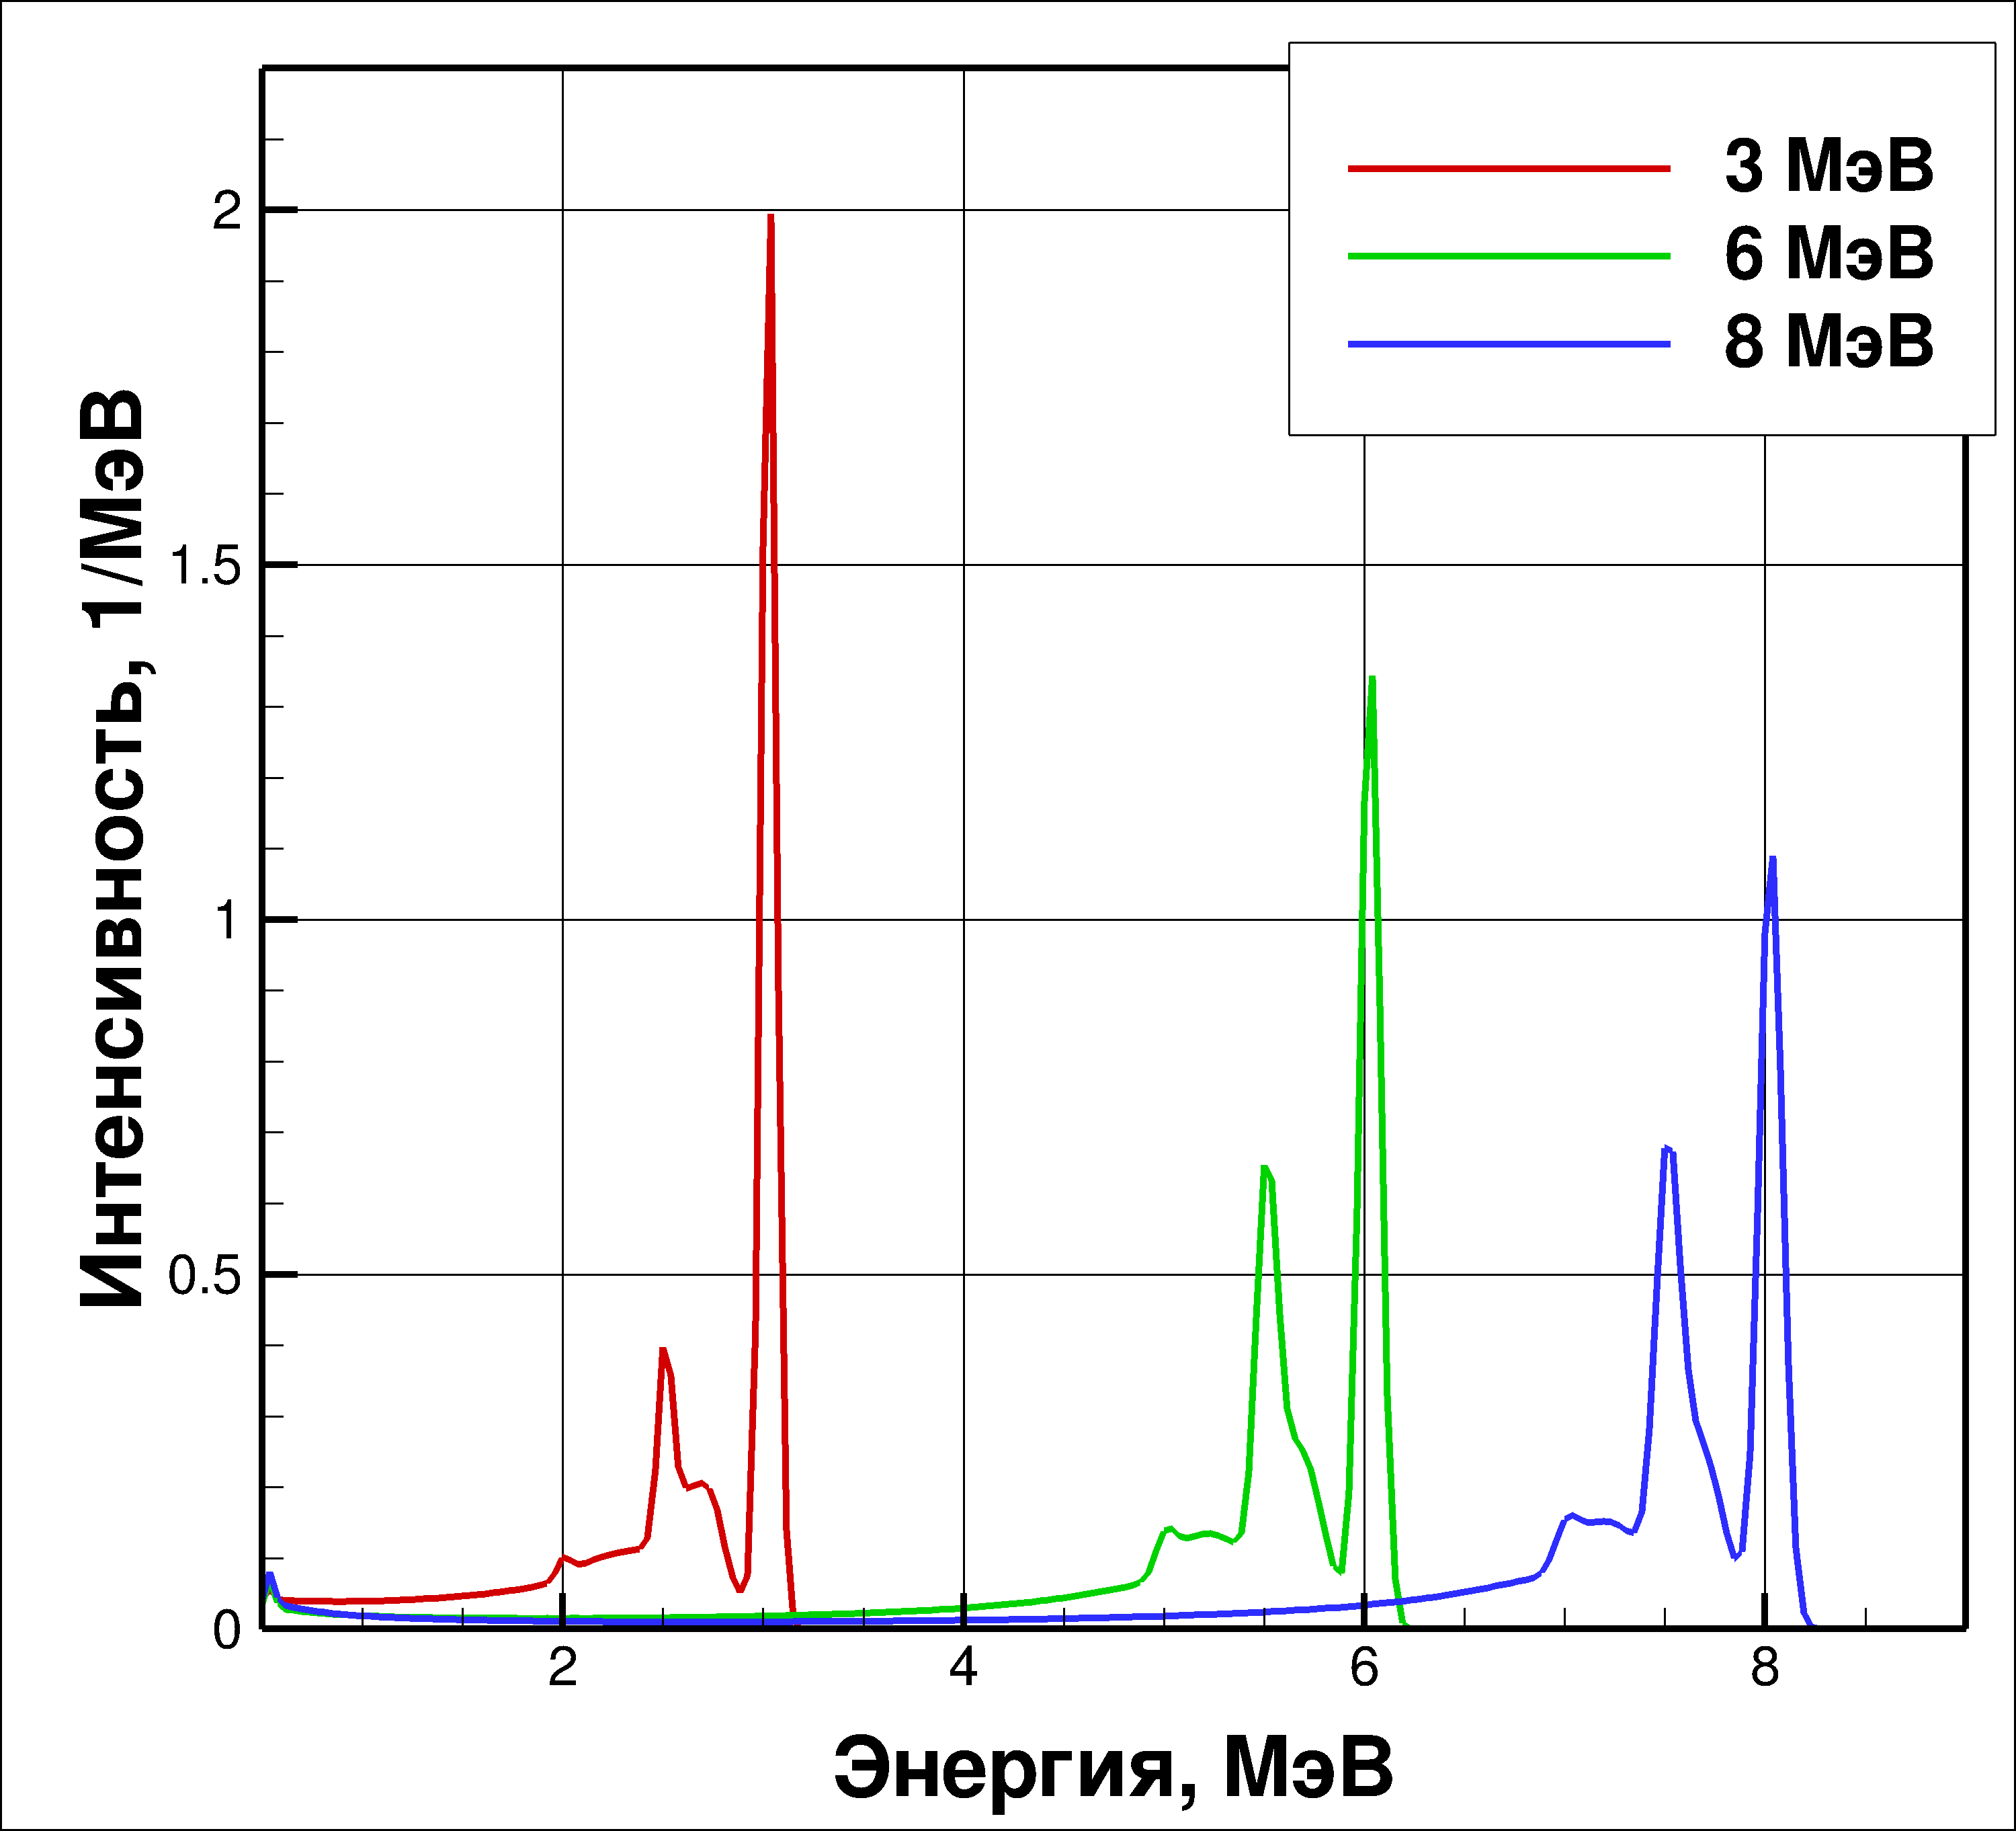
\includegraphics[width=0.52\linewidth]{mcnpInstFunctionsNaI} }
  \caption{ Примеры аппаратных функций, рассчитанных с помощью кода MCNP для детектора NaI(Tl) для различных значений энергии поглощаемых гамма квантов.~\cite{Shevelev2013} }
  \label{fig:mcnpInstFunctionsNaI}
\end{figure}

Были проведены измерения с использованием детектора NaI(Tl) размером $\varnothing$150$\times$100~мм с энергетическим разрешением 11,5\% на линии 661.6~кэВ. Функции отклика этого детектора рассчитывались по программе MCNP в диапазоне энергий 60--3000~кэВ с шагом 20~кэВ; расчёты выполнял А.~Е.~Шевелев. В разработанной расчетной модели источник изотропного гамма-излучения располагался на расстоянии 25.5~см от детектора. На одинаковом расстоянии от реального детектора для проведения измерений были установлены радиоактивные источники ${}^{60}$Co и ${}^{137}$Cs с известной активностью распада. Результаты обработки измеренного спектра показаны на рисунке~\ref{fig:cocsReconstructIoffe}. Время набора первого спектра составляет 150~секунд, время набора второго спектра --- 2~секунды, оба спектра были набраны в одинаковой геометрии. Обработка второго спектра иллюстрирует способность алгоритма работать с данными с низкой статистикой. Количество событий в восстановленных пиках соответствует количеству гамма-квантов, испущенных радиоактивными источниками во время регистрации спектра. Применяемая методика позволила определить активность радиоактивных источников с точностью 1.5\% для спектра с временем набора 150~секунд и 2.4\% для спектра с временем набора 2~секунды.~\cite{Shevelev2013}

\begin{figure}[ht!]
    \begin{minipage}[b][][b]{0.95\linewidth}\centering
        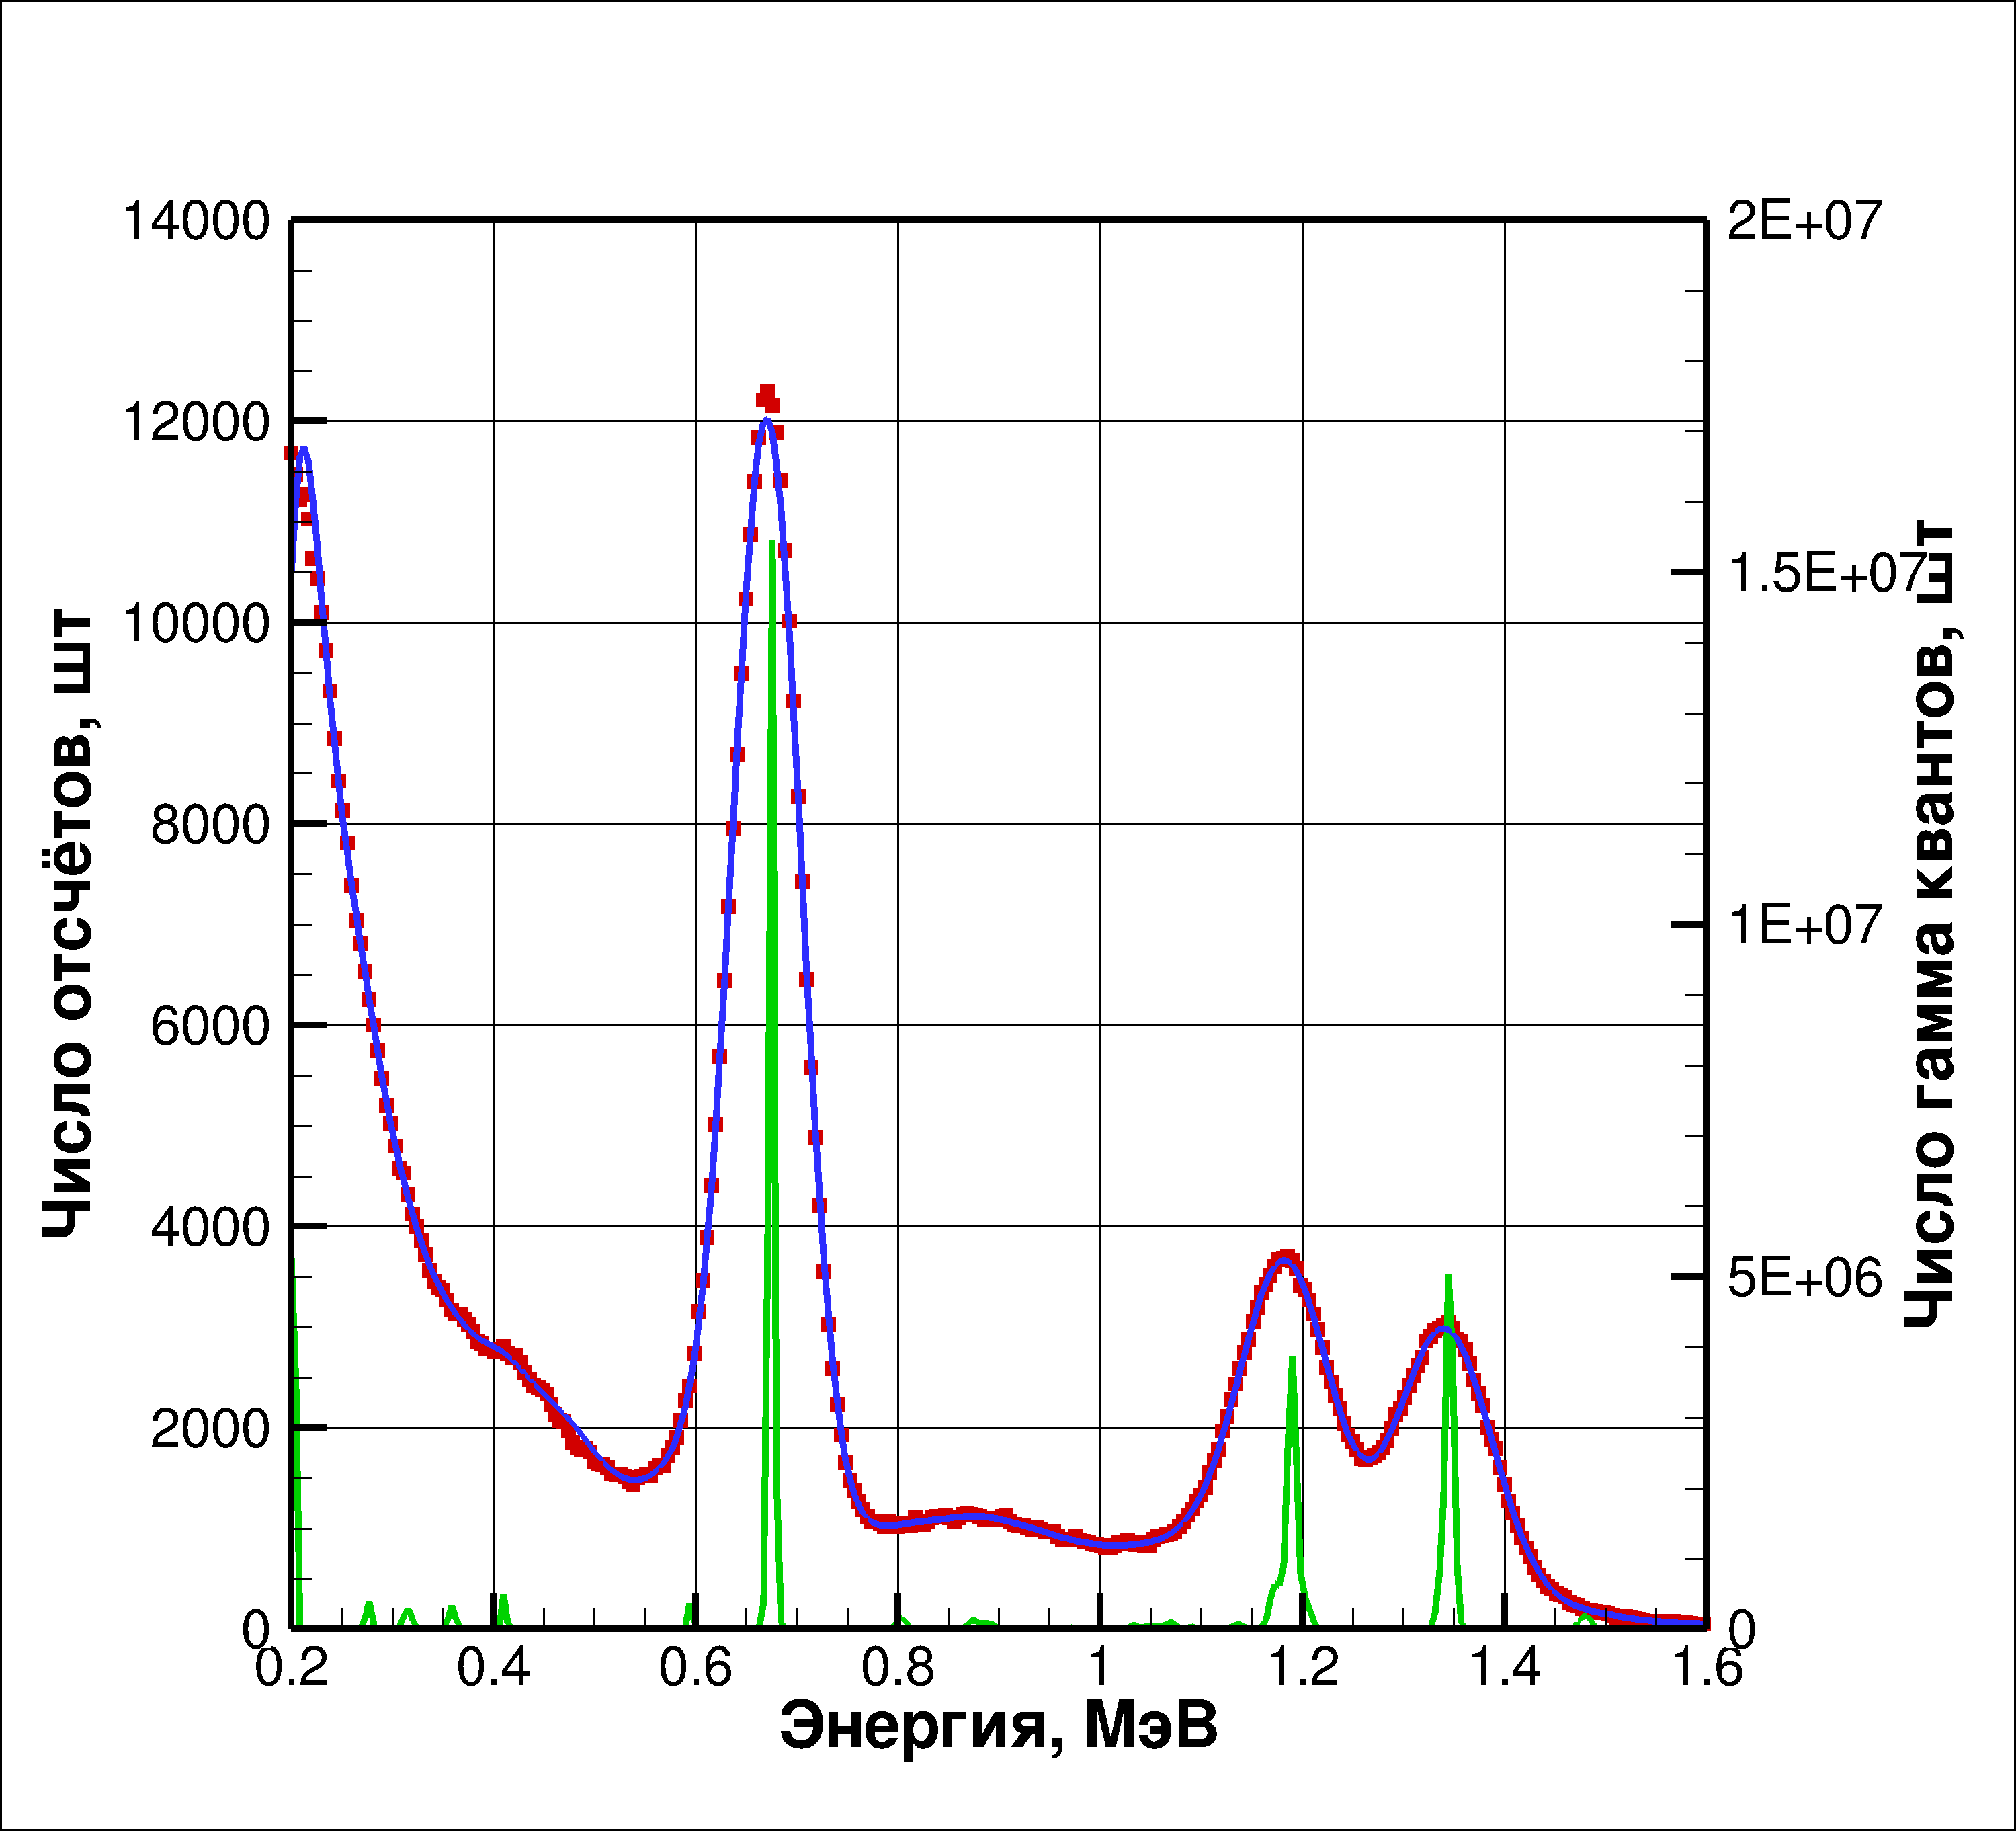
\includegraphics[width=0.52\linewidth]{cocsReconstructIoffe300s} \\ а) \\
    \end{minipage}
    \vfill
    \begin{minipage}[b][][b]{0.95\linewidth}\centering
        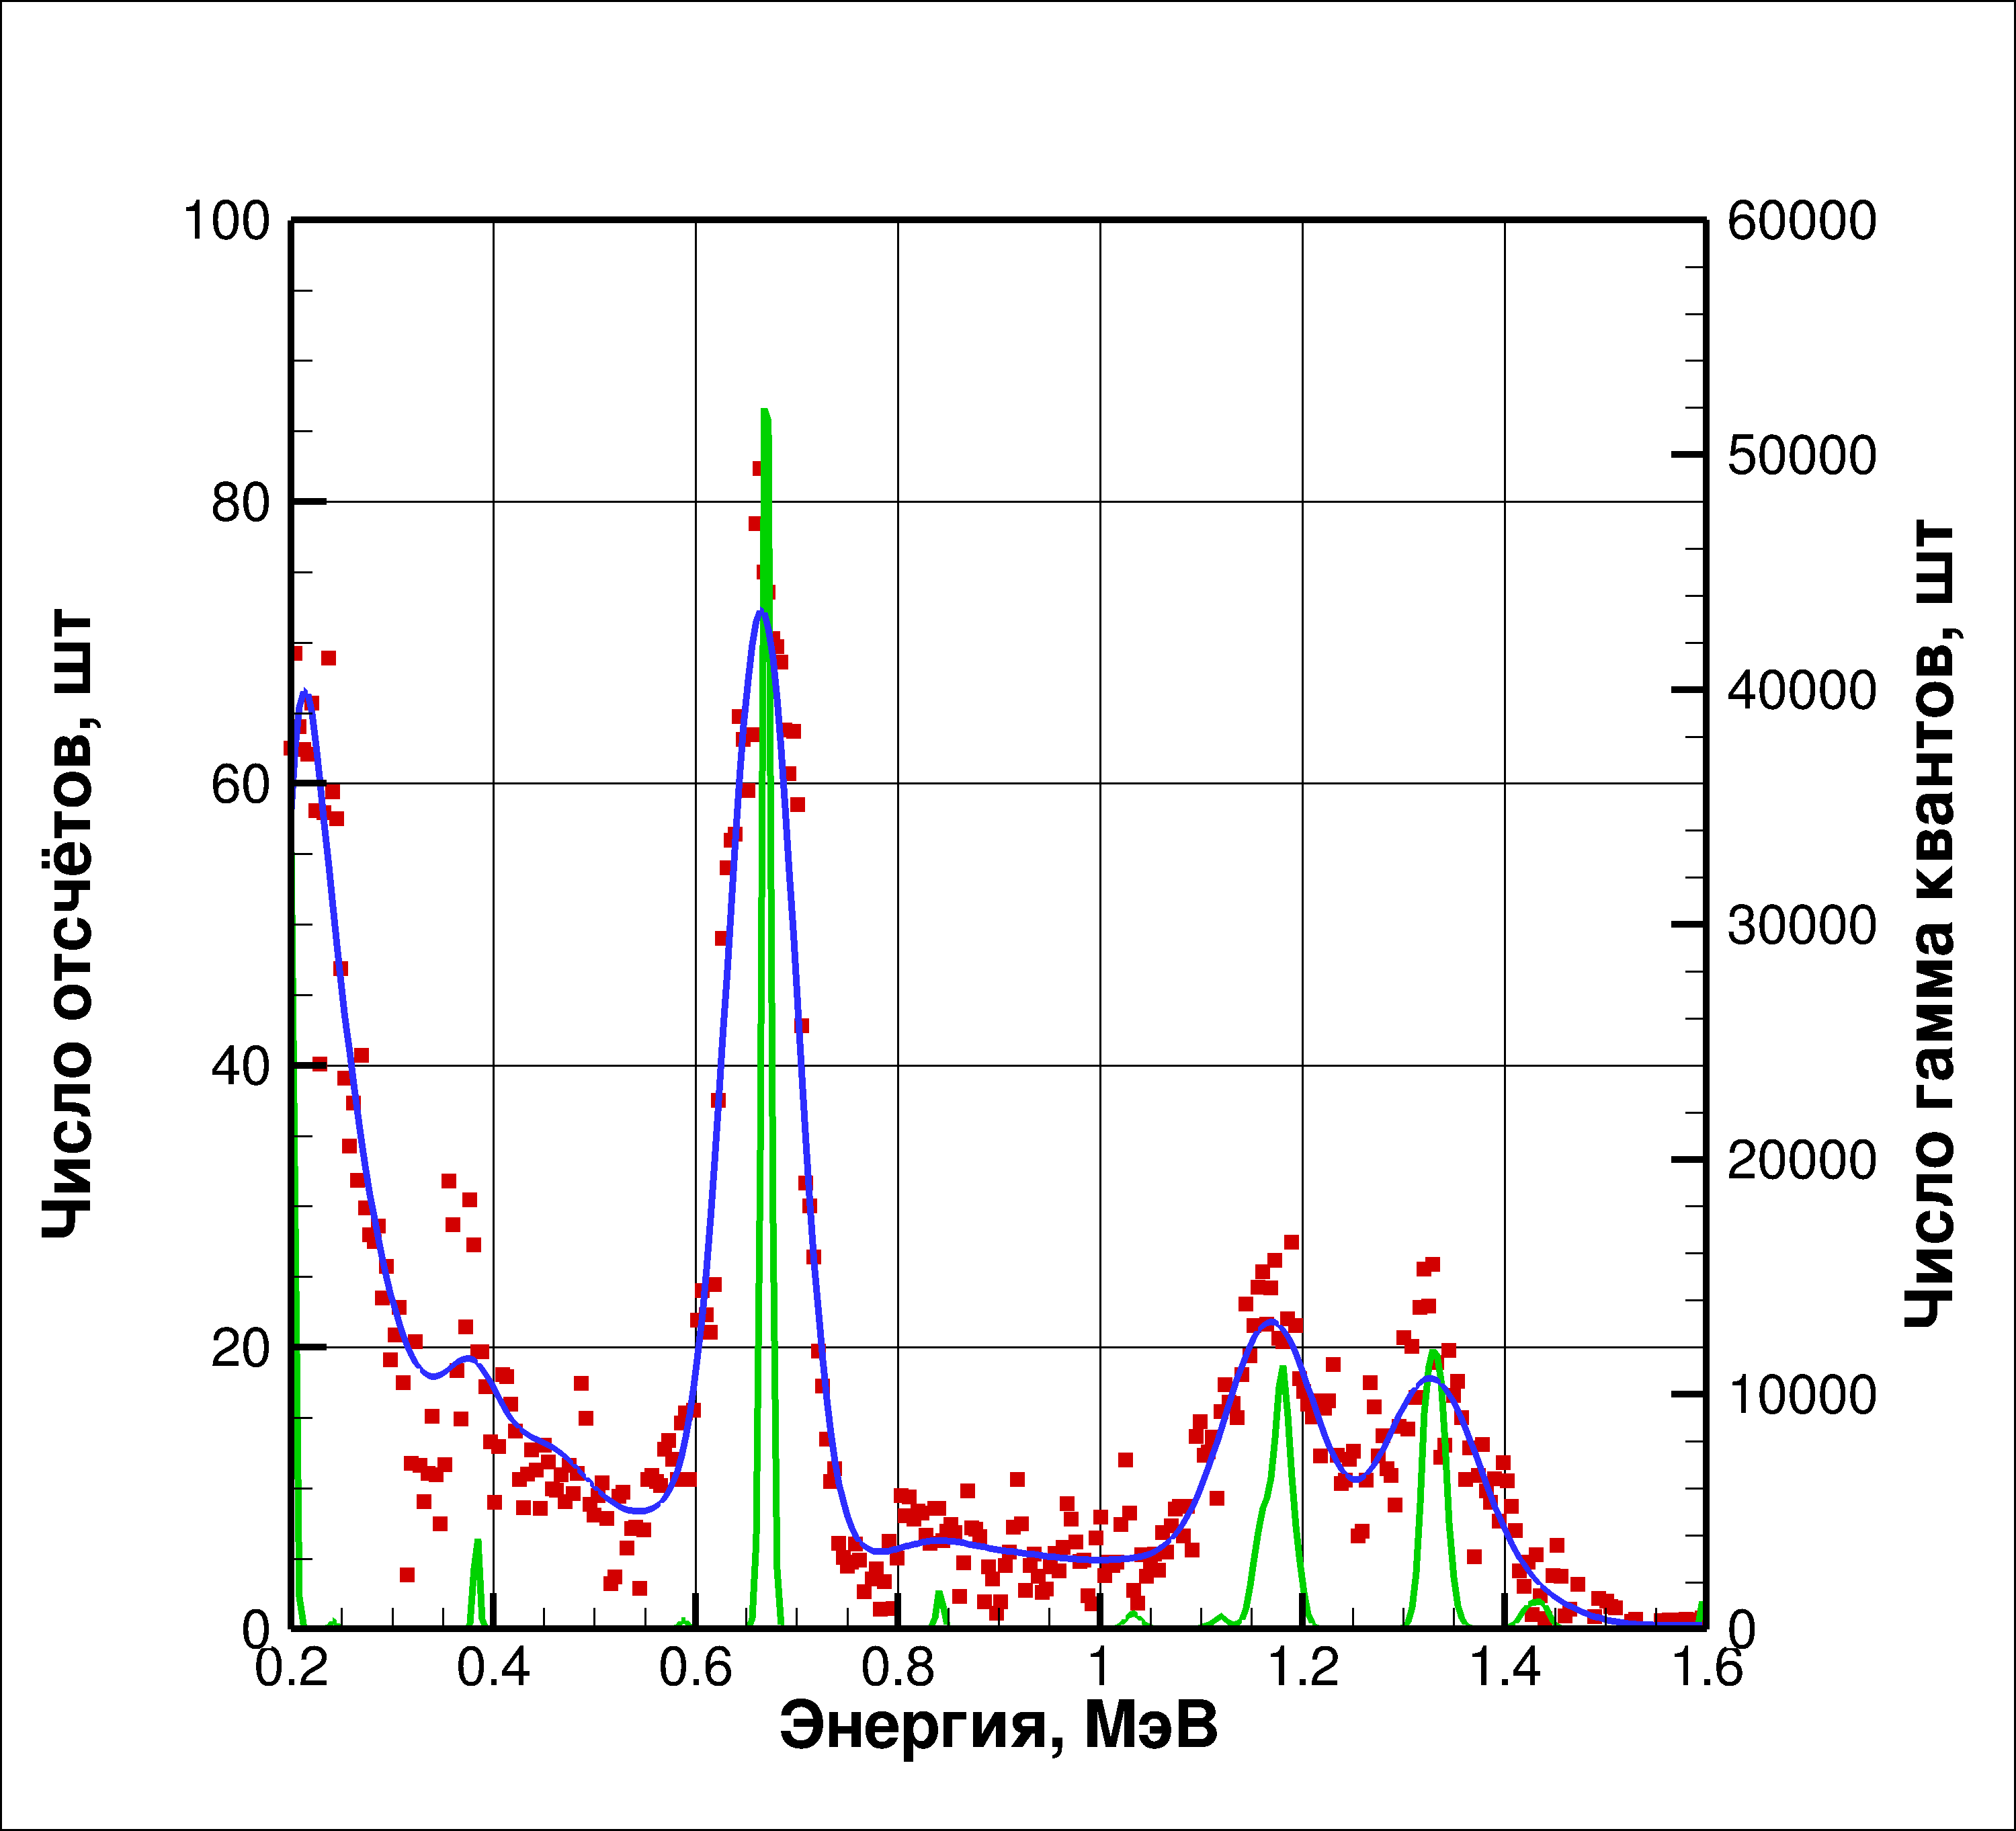
\includegraphics[width=0.52\linewidth]{cocsReconstructIoffe2s} \\ б) \\
    \end{minipage}
    \vspace{5mm}
    \caption{ Спектр источников ${}^{60}$Co и ${}^{137}$Cs, время набора 150 секунд (а) и 2 секунды (б). Красной линией показан измеренный детектором спектр, зелйной линией --- восстановленный спектр источников гамма излучения, синим --- результат <<прямой свёртки>>, интегрирования восстановленного спектра с передаточной функцией детектора (аппаратной функцией с учётом геометрии источника и детектора). В случае идеального восстановления спектра синяя кривая должна совпадать с красными точками.~\cite{Shevelev2013}. }
    \label{fig:cocsReconstructIoffe}
\end{figure}
\FloatBarrier

В другом эксперименте в измерениях использовался тот же самый NaI(Tl) детектор с размерами $\varnothing$150$\times$100~мм. Использовался источник гамма-излучения ${}^{152}$Eu с известной активностью распада. Результат обработки спектра источника ${}^{152}$Eu показан на рисунке~\ref{fig:euReconstructedSpectrum} и в таблице~\ref{tab:euReconstructedLines}. Из этого спектра был предварительно вычтен измеренный спектр фонового излучения. Восстановленный спектр позволил определить все основные линии источника ${}^{152}$Eu. Ошибка определения линий с высокой интенсивностью оказывается сравнительно небольшой. Она может быть объяснена  неточным  определением расстояния до источника. Метод позволил выявить линии с крайне малой интенсивностью 1.212~МэВ, 1.299~МэВ, 0.688~МэВ, 0.586~МэВ, 0.563~МэВ, невидимые в исходном спектре, хотя и с большой относительной ошибкой при определении амплитуды. Удалось обнаружить так же невидимую в исходном спектре линию 0.867~МэВ и сравнительно точно определить её интенсивность. Удалось разрешить близко расположенные пары линий 0.411 и 0.444~МэВ, 1.085 и 1.112~МэВ.~\cite{Khilkevitch2013}

\begin{figure}[ht!]
  \centerfloat{ 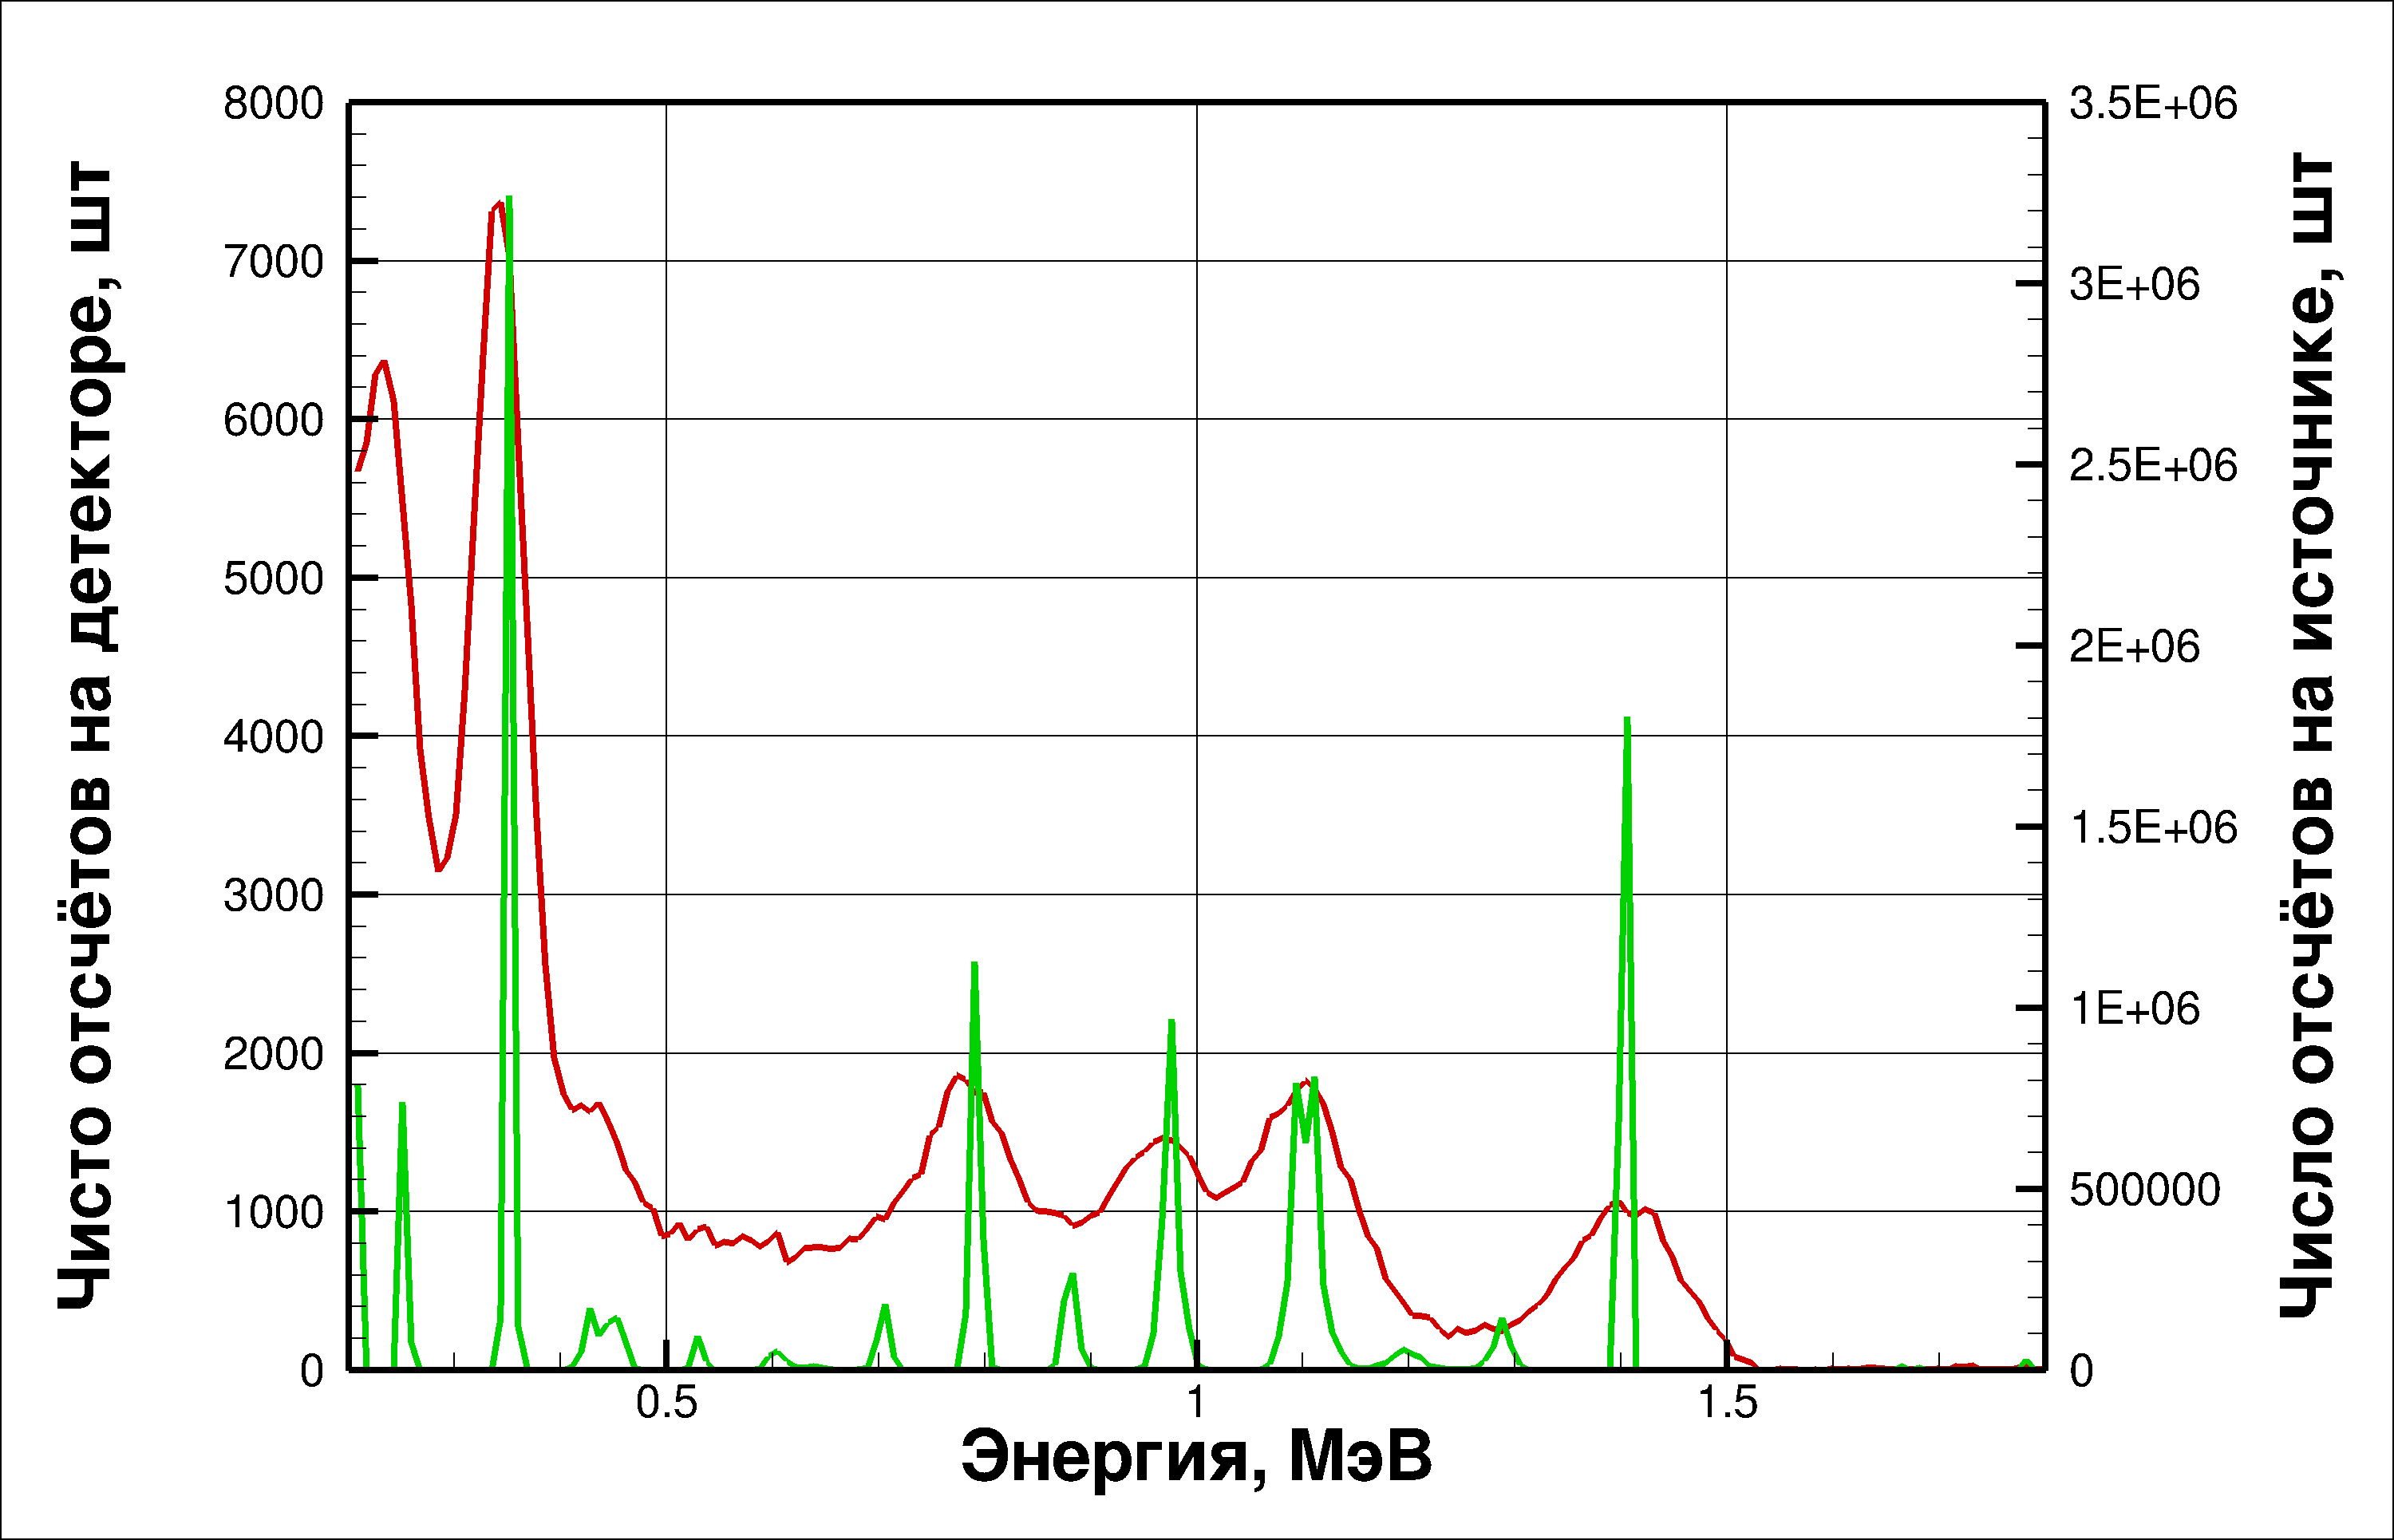
\includegraphics[width=0.52\linewidth]{euReconstructedSpectrum} }
  \caption{ Восстановленный спектр излучения источника ${}^{152}$Eu после вычитания фона. Время набора спектра --- 300 секунд. Красная линия --- измеренный спектр (отсчёты по левой оси), зелёная линия --- восстановленный спектр (отсчёты по правой оси).~\cite{Khilkevitch2013} }
  \label{fig:euReconstructedSpectrum}
\end{figure}

\begin{table}[htbp]
    \centering
    \begin{threeparttable}
      \caption{ Интенсивности и энергии пиков восстановленного спектра источника ${}^{152}$Eu. Интенсивность линий из паспорта представляет собой сумму линий с большой интенсивностью и рядом находящихся линий малой интенсивности (менее 1\%).~\cite{Khilkevitch2013} }
        \label{tab:euReconstructedLines}
        \begin{tabular}{| p{1cm} | p{3.5cm} | p{3.5cm} | p{3.5cm} | p{3.5cm} | }
            \hline
            \makecell{\textnumero} & \makecell{ Энергия линий \\ по паспорту, \\ МэВ } & \makecell{ Энергия \\ восстановлен-\\ных линий, МэВ } & 
                \makecell{Интенсивность \\ по паспорту, c${}^{-1}$} & \makecell{Восстанов-\\ленная \\ интенсив-\\ность, c${}^{-1}$ } \\
            \hline
             1 & 0.245 & 0.243 & 3018 & 2722 \\
             2 & 0.344 & 0.349 & 11115 & 11683 \\
             3 & 0.411 & 0.428 & 945 & 994 \\
             4 & 0.444 & 0.453 & 1269 & 1300 \\
             5 & 0.563 & 0.529 & 447 & 411 \\
             6 & 0.586 & 0.604 & 367 & 441 \\
             7 & 0.688 & 0.706 & 863 & 1033 \\
             8 & 0.778 & 0.790 & 5585 & 5529 \\
             9 & 0.867 & 0.883 & 1841 & 1800 \\
             10 & 0.964 & 0.975 & 6229 & 6316 \\
             11 & 1.085 & 1.035 & 4815 & 4392 \\
             12 & 1.112 & 1.111 & 5501 & 5326 \\
             13 & 1.212 & 1.195 & 673 & 653 \\
             14 & 1.299 & 1.288 & 710 & 1083 \\
             15 & 1.408 & 1.406 & 8469 & 8257 \\
            \hline
        \end{tabular}
    \end{threeparttable}
\end{table}

% ==========================================================

\FloatBarrier
\section{ Восстановление функции распределения убегающих электронов по измеренному спектру излучения }

\subsection{ Использование метода ML-EM для восстановления функции распределения убегающих электронов }
\label{sec:runawayReconstructionMlem}

При торможении электрон испускает поток квантов жёсткого рентгеновского излучения, которое может быть зарегистрировано гамма детекторов. Спектр рентгеновского излучения имеет почти непрерывный характер; максимальная энергия рождённых квантов равна кинетической энергии электрона, однако вероятность рождения единственного кванта с максимальной энергией не велика, большая часть спектра излучения приходится на меньшие энергии.~\cite{Kuznetsov1974}

Спектр рентгеновского излучения, генерируемый в процессе торможения электронов, может быть описан следующей формулой:
\begin{equation}
  \label{eq:RunawayConvolution}
  g( \varepsilon ) = \int \limits_0^{ \varepsilon } f(\varepsilon') k( \varepsilon, \varepsilon' ) d \varepsilon'
\end{equation}
где $f(\varepsilon)$ --- функция распределения электронов по энергии, $k( \varepsilon, \varepsilon' )$ --- функция генерации излучения убегающими электронами. Для моноэнергетического пучка электронов с энергией $\varepsilon_0$ и интенсивностью $I$, то есть $ f(\varepsilon) = I \cdot \delta( \varepsilon - \varepsilon_0 ) $, спектр тормозного рентгеновского излучения будет равен $g(\varepsilon) = I \cdot k( \varepsilon, \varepsilon_0 )$. Очевидно что при всех значениях $\varepsilon > \varepsilon'$ значения $k( \varepsilon, \varepsilon' ) = 0$, поскольку электрон не в состоянии сгенерировать гамма квант с энергией больше, чем энергия электрона.~\cite{Shevelev2013} 

Функция $k( \varepsilon, \varepsilon' )$ может быть рассчитана с помощью кода MCNP. Она зависит от угла между линией наблюдения и угловым распределением направления движения электронов, а так же от материала, на котором происходит торможение. Интенсивность излучения оказывается пропорциональна квадрату заряда ядер, на которых происходит рассеяние, а диаграмма углового распределения излучения имеет явно выраженную анизотропию в направлении налетающего пучка электронов.~\cite{Shevelev2013}

Уравнение~\ref{eq:RunawayConvolution} можно подставить в~\ref{eq:BaseConvolution}, тогда:
\begin{equation}
  \label{eq:RunawayBaseConvolution}
  \begin{alignedat}{1}
    s( \varepsilon ) = & \int \limits_0^{+\infty} d \varepsilon' h( \varepsilon, \varepsilon' ) \int \limits_0^{\varepsilon'} d \varepsilon'' f( \varepsilon'') k( \varepsilon', \varepsilon'' ) + n(\varepsilon) \\
    = & \int \limits_0^{+\infty} d \varepsilon'' f( \varepsilon'' ) \int \limits_0^{+\infty} d \varepsilon' h( \varepsilon, \varepsilon' ) k( \varepsilon', \varepsilon'' ) + n(\varepsilon) \\ 
    = & \int \limits_0^{+\infty} d \varepsilon'' f( \varepsilon'' ) h^{tot}( \varepsilon, \varepsilon'' ) + n(\varepsilon)
  \end{alignedat}  
\end{equation}
где $h^{tot}( \varepsilon, \varepsilon'' )$ --- свёртка функций отклика из уравнения~\ref{eq:RunawayConvolution} с передаточной функцией из уравнения~\ref{eq:BaseConvolution}. Вид этого уравнения полностью совпадает с видом уравнения~\ref{eq:BaseConvolution}, и далее для решения уравнения~\ref{eq:RunawayBaseConvolution} можно применять описанный выше метод ML-EM. В связи с характером искомого решения нецелесообразно использовать возведение в степень для вытягивания пиков (уравнение~\ref{eq:BoostMlemDisturb}), но целесообразно чаще применять процедуру сглаживания. Ошибку восстановления функции распределеня можно проводить описанным выше методом Монте-Карло.~\cite{Shevelev2013}

% ----------------------------------------------------------

\subsection{Определение максимальной энергии убегающих электронов}

По итогам восстановления функции распределения обычно имеет ненулевое значение во всём диапазоне энергий; однако в тех диапазонах энергий, где функция электронов фактически равна нулю, значение вычисленной восстановленной функции распределения оказывается близка к нулю с точностью до машинной погрешности, то есть на 10--14 порядков меньше, чем значение функции распределения в её максимуме. Поскольку в правой части функции распределения наблюдается спад значений функции к ненулевому значению, встаёт вопрос о том, какую именно энергию выбирать в качестве максимальной энергии убегающих электронов. Очевидно, что фактически такая энергия имеет физический смысл согласно уравнению~\ref{eq:MaxRunawayEnergyLimit} (в отличие например от максвелловского распределения, где понятие максимальной энергии не имеет строгого физического смысла). 

Предлагается для поиска максимальной энергии найти такое значение $\varepsilon_{max}$, что
\begin{equation}
  \label{eq:RunawayMaxEnergy}
  \rho = 1 - \frac{ \int \limits_{\varepsilon_0}^{\varepsilon_{max}} f(\varepsilon) d\varepsilon }{ \int \limits_{\varepsilon_0}^{+\infty} f(\varepsilon) d\varepsilon }
\end{equation}
где значение $\rho$ --- параметр, равный например $10^{-3}$. Значение начальной энергии интегрирования $\varepsilon_0$ ненулвевое, потому что в некоторых ситуациях функция распределения убегающих электронов очень сильно возрастает вблизи нуля, что приводит к сильной зависимости результата вычисления от порога. Обычно значение $\varepsilon_0$ имеет смысл выбирать в районе 1--2~МэВ. По физическому смыслу формулы~\ref{eq:RunawayMaxEnergy} больше выбранной максимальной энергии $\varepsilon_{max}$ на функции распределения находится статистически незначительное число электронов. Как показывает практика, значение $\varepsilon_{max}$ очень слабо зависит от произвольно выбираемых параметров $\rho$ и $\varepsilon_0$, поскольку обычно правый край полученной функции распределения имеет крутой правый край. Крутизна этого края определяется как физическими процессами, так и является следствием применения процедуры сглаживания, которая применяется при восстановлении функции распределения.~\cite{Shevelev2017}

% ----------------------------------------------------------

\subsection{ Проверка корректности восстановления и отработка методики восстановления функции распределения убегающих электронов по энергии на модельных спектрах }

Если для тестирования процедуры восстановления дискретного спектра можно использовать калибровочные источники гамма излучения, то для тестирования восстановления функции распределения убегающих электронов подобный удобный тестовый объект с известным распределением в нашем распоряжении отсутствует. Поэтому для проверки были использованы сгенерированные и обработаны модельные сигналы.

Для тестирования с помощью кода MCNP с учетом положения детектора NaI(Tl) в Roof lab с вертикальной линией обзора на токамаке JET были рассчитаны спектры тормозного излучения, соответствующие потокам жёсткого рентгена от моноэнергетических электронов в средней плоскости вакуумной камеры. Некоторые из этих спектров показаны на рисунке~\ref{fig:mcnpRunawayResponseJetSh2013}. В модели пучок ускоренных электронов с заданным распределением энергии в экваториальной плоскости корпуса JET взаимодействует с объемными ионами. Расчеты проводились в геометрии вакуумной камеры токамака JET для дейтериевой плазмы с плотностью электронов $ 5 \cdot 10^{19}$~м${}^{-3}$ и 2\% примеси углерода. Расчёты выполнены А.~Шевелевым.~\cite{Shevelev2013} 

\begin{figure}[ht!]
  \centerfloat{ 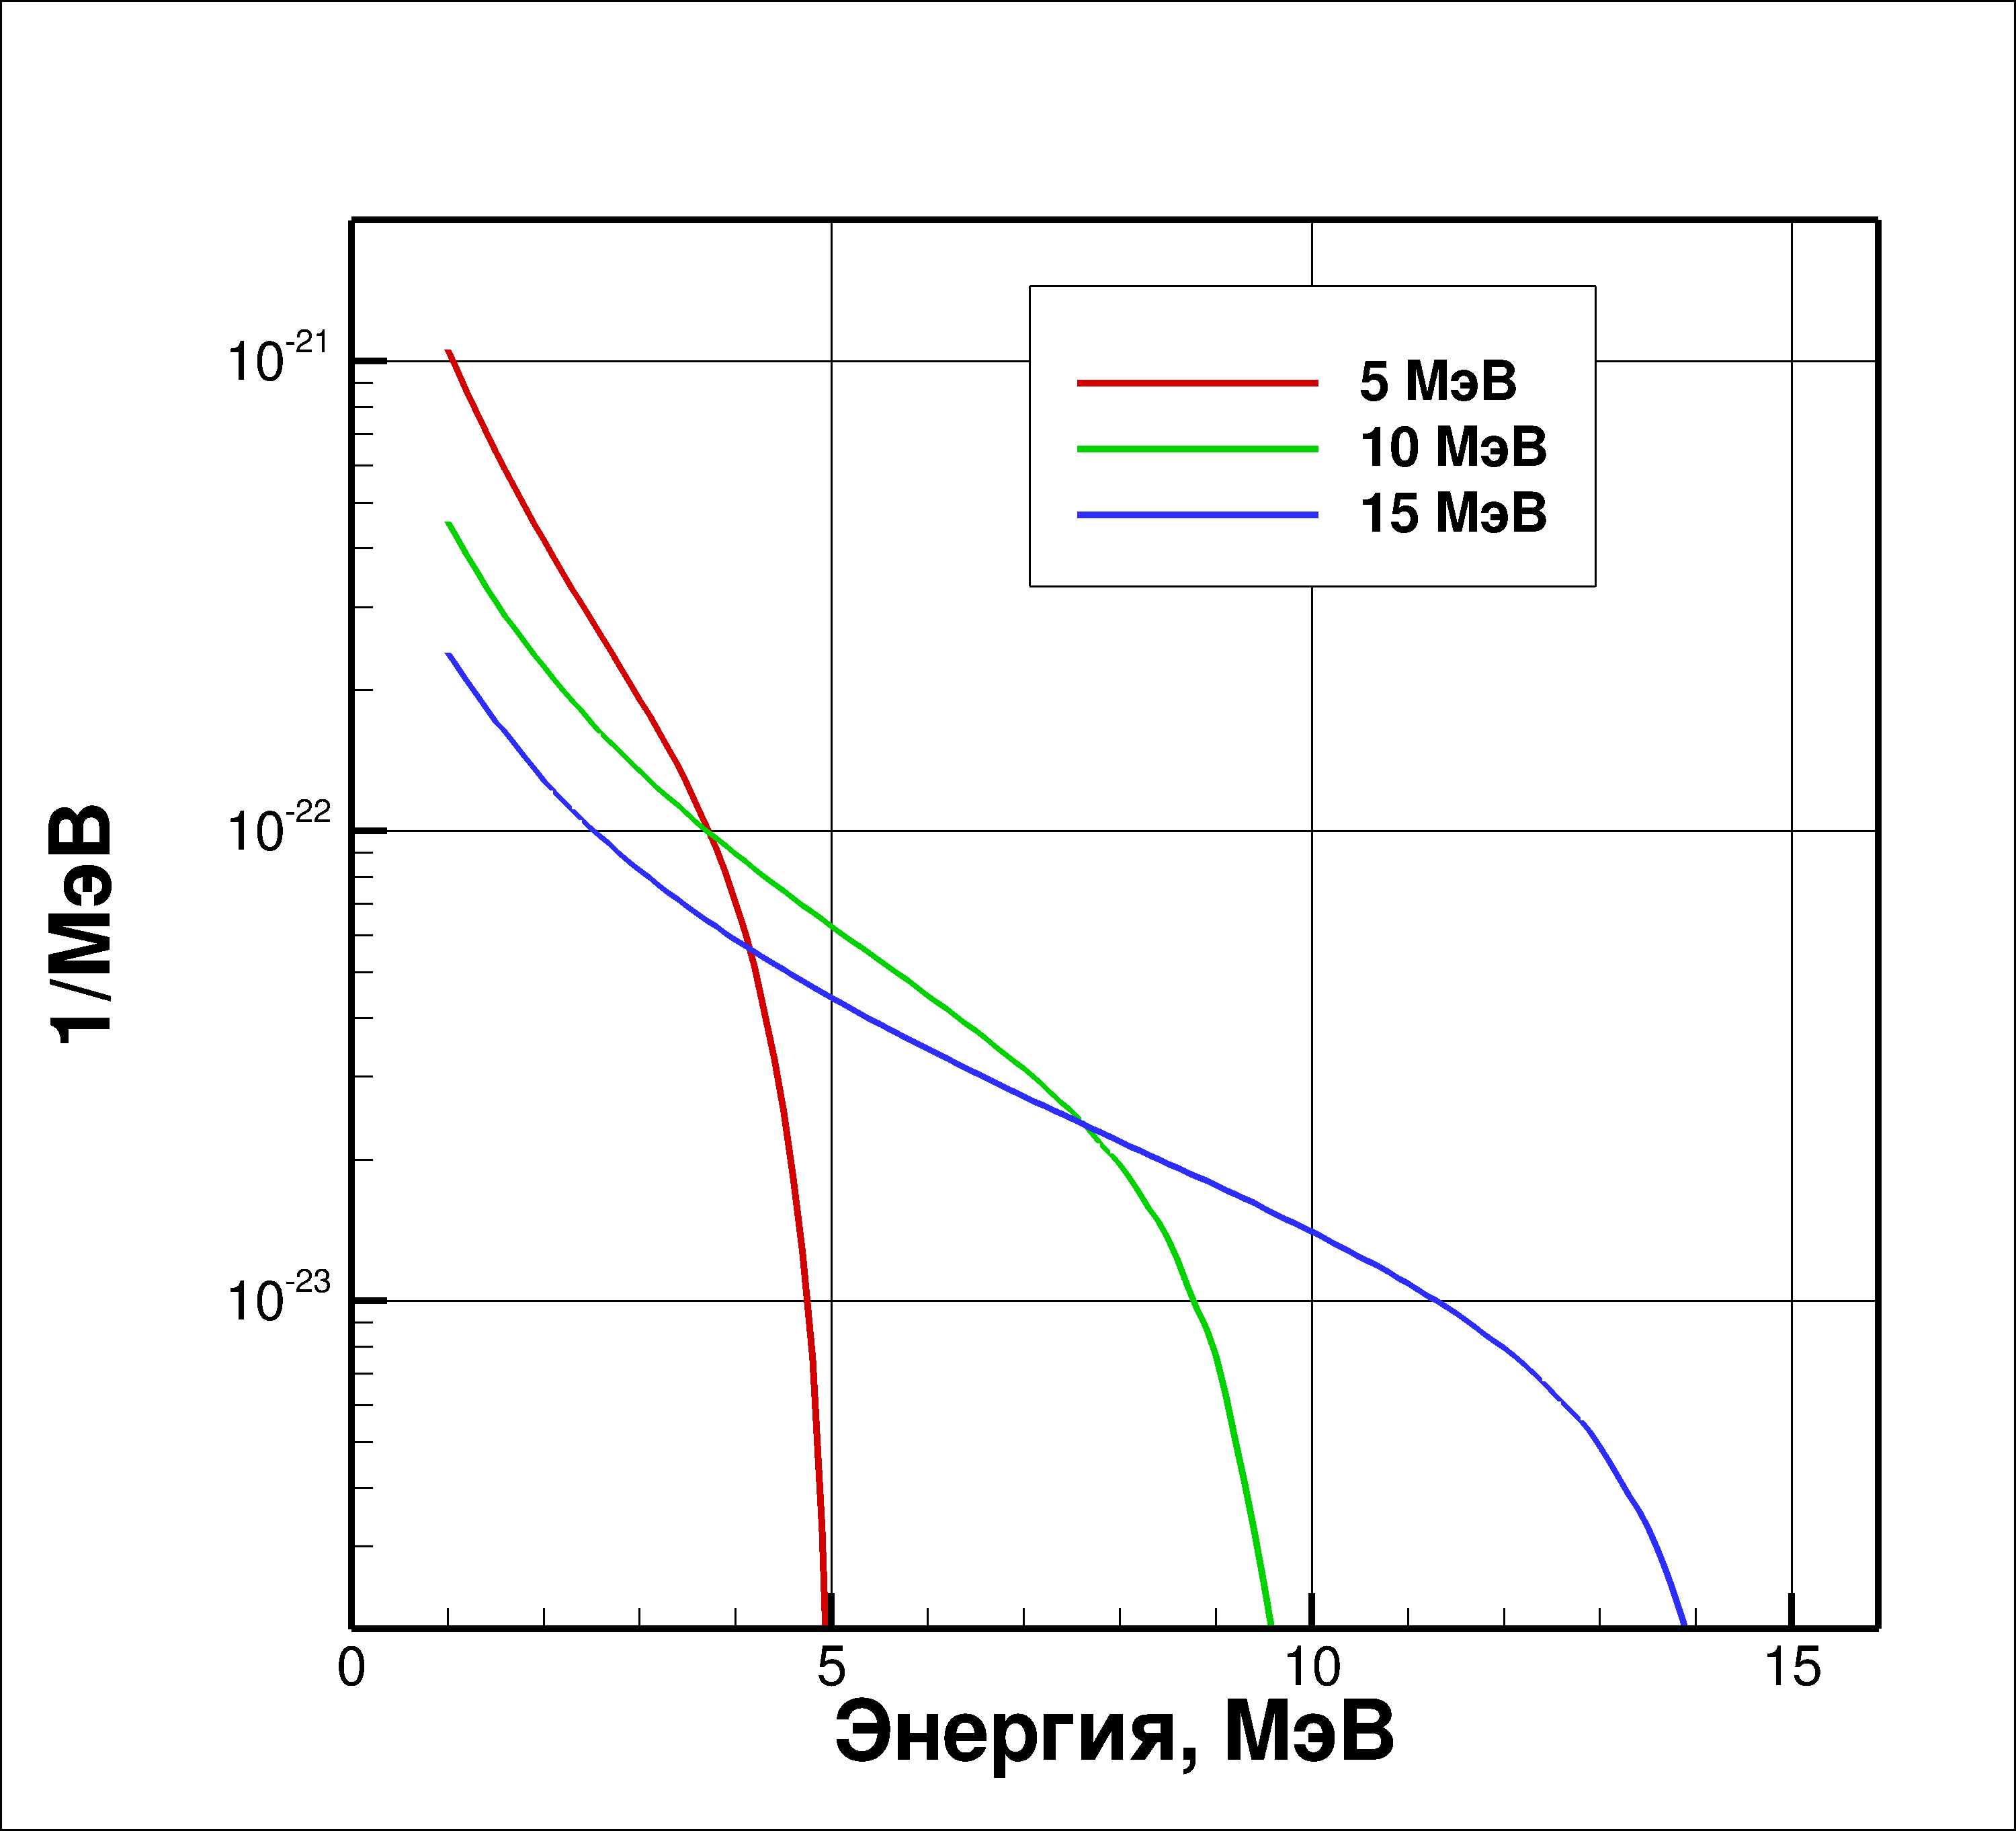
\includegraphics[width=0.52\linewidth]{mcnpRunawayResponseJetSh2013} }
  \caption{ Спектры жёсткого рентгеновского излучения, генерируемые убегающими электронами с энергиями 5, 10, 15~МэВ, рассчитанные с помощью кода MCNP. Расчёт проведён для условий токамака JET.~\cite{Shevelev2013} }
  \label{fig:mcnpRunawayResponseJetSh2013}
\end{figure}

Распределение энергии электронов, используемое в моделировании, показано на рисунке~\ref{fig:runawayJetSimulationEdfSh2013} зеленой линией с широким пиком в области высоких энергий. Такая форма распределения вполне реальна при наличии первичных и вторичных механизмов генерации убегающих электронов, а также в условиях, ограничивающих неуправляемый рост энергии, например, за счет потерь на синхротронное излучение~\cite{MartinSolis1999,Shevelev2013}. Интеграл по  распределению равен числу электронов, прошедших через видимый объем плазмы. По этой функции распределения с использованием функции генерации, изображённой на рисунке~\ref{fig:mcnpRunawayResponseJetSh2013} и с использованием функции, изображённой на рисунке~\ref{fig:mcnpInstFunctionsNaI} был построен спектр жёсткого рентгеновского излучения, который регистрируется детектором. Этот спектр изображён зелёными точками на рисунке~\ref{fig:runawayJetSimulationSpectrumSh2013}. На спектр был наложен шум, соответствующий пуассновской статистике.~\cite{Shevelev2013}

\begin{figure}[ht!]
  \centerfloat{ 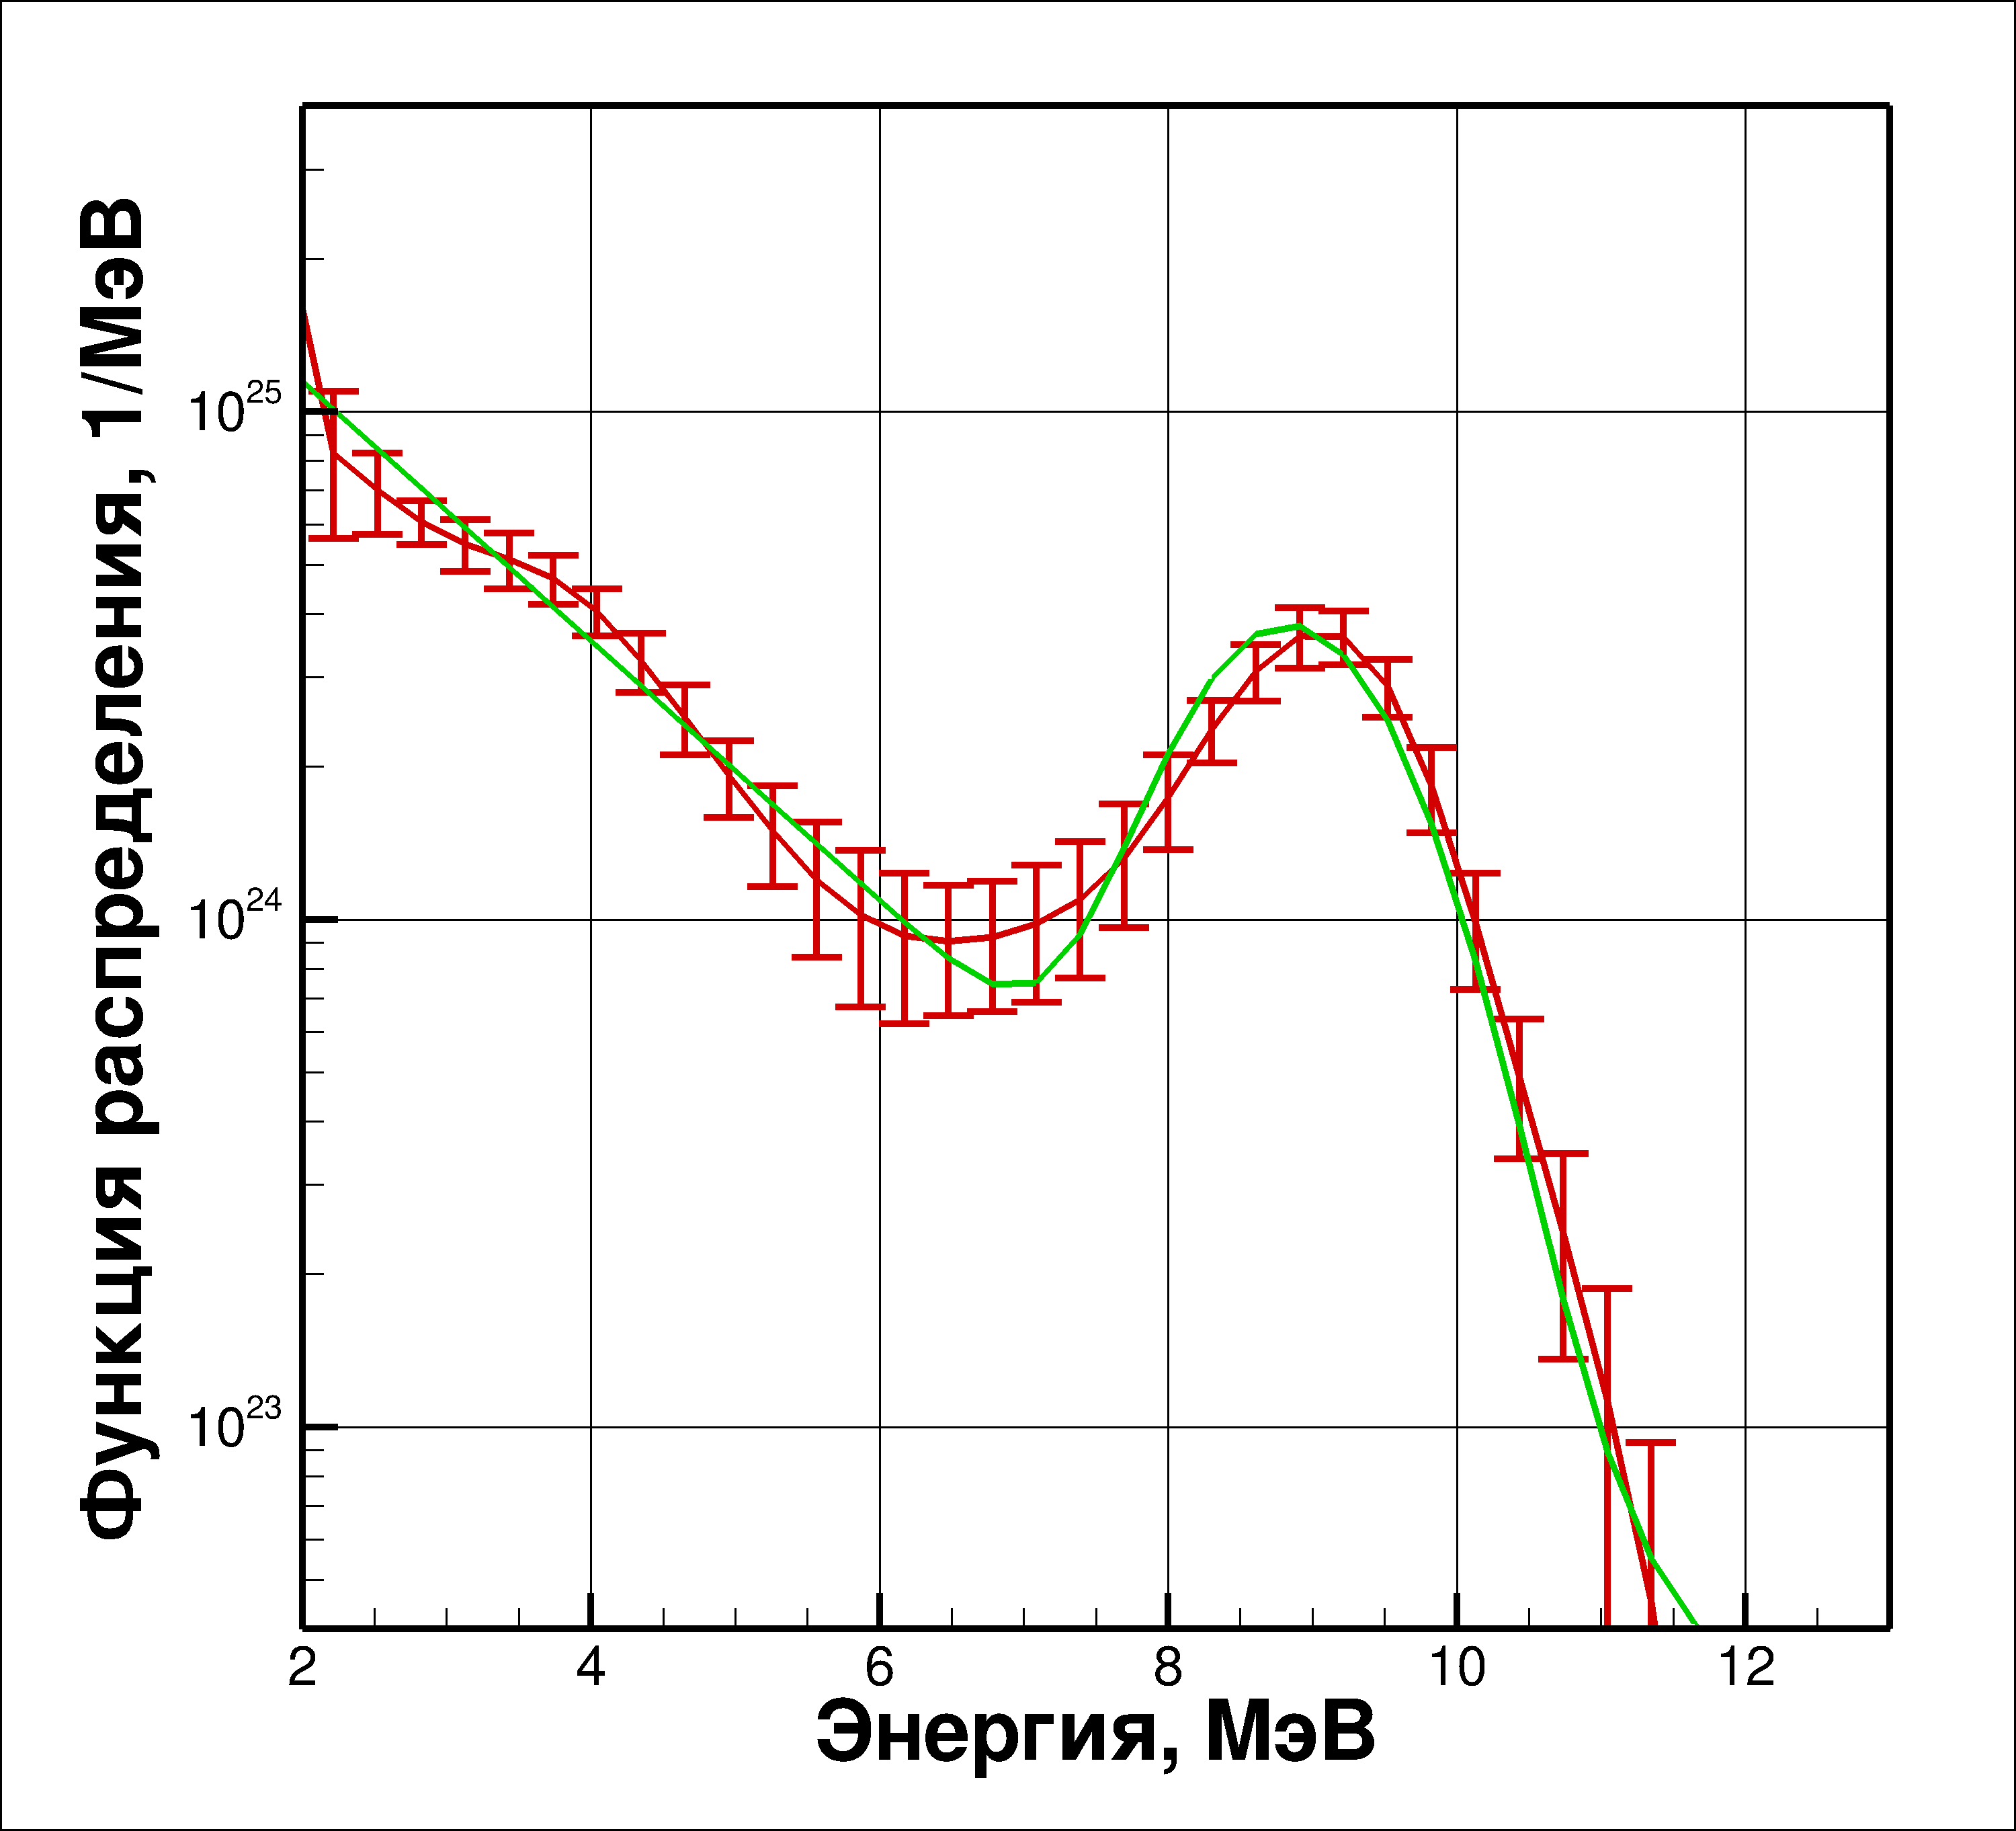
\includegraphics[width=0.52\linewidth]{runawayJetSimulationEdfSh2013} }
  \caption{ Функции распределения убегающих электронов: зелёным цветом показана сгеренированая функция распределения, красным --- восстановленная.~\cite{Shevelev2013} }
  \label{fig:runawayJetSimulationEdfSh2013}
\end{figure}

\begin{figure}[ht!]
  \centerfloat{ 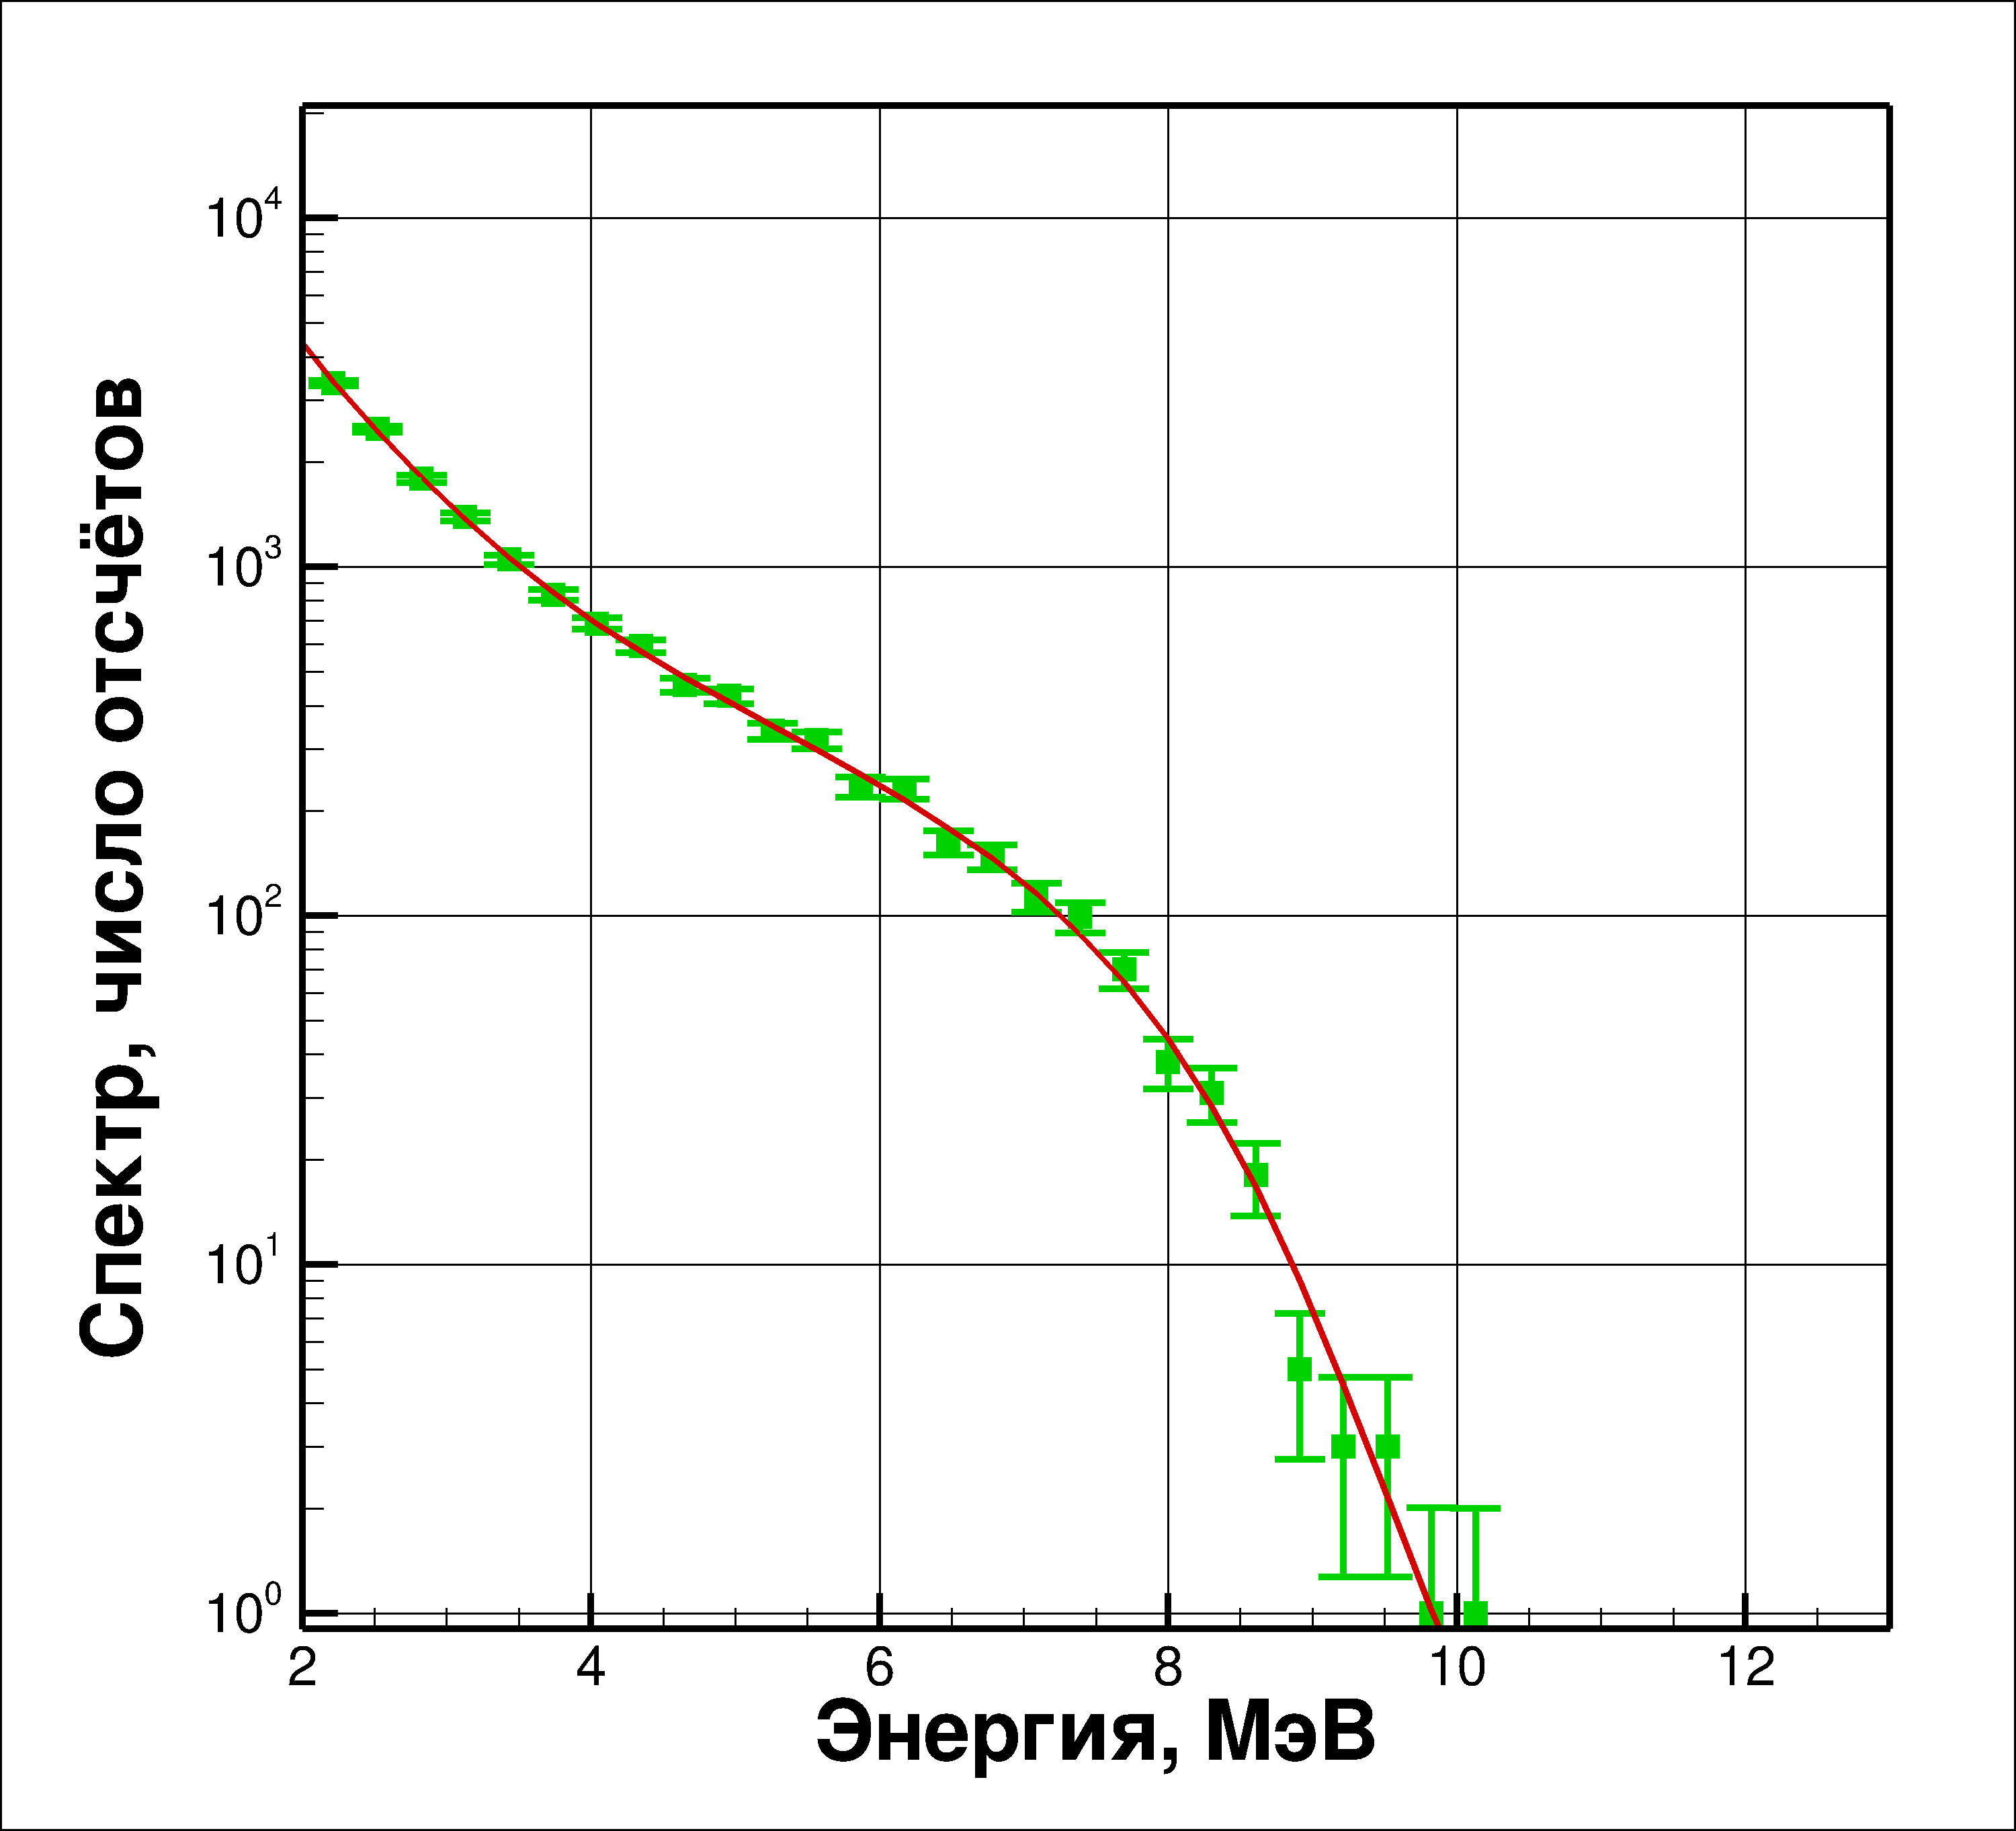
\includegraphics[width=0.52\linewidth]{runawayJetSimulationSpectrumSh2013} }
  \caption{ Спектр жёсткого рентгеновского излучения: зелёным цветом показан спектр, соответствующий сгенерированной функции распределения с рисунка~\ref{fig:runawayJetSimulationEdfSh2013}, полученный по формуле~\ref{eq:RunawayBaseConvolution}, красным цветом показан спектр, соответствующий восстановленной функции распределения с того же рисунка.~\cite{Shevelev2013} }
  \label{fig:runawayJetSimulationSpectrumSh2013}
\end{figure}

К сгеренрированному спектру была применена описанная в разделе~\ref{sec:runawayReconstructionMlem} процедура восстановления функции распределения убегающих электронов по энергии. Результат восстановления показан на рисунке~\ref{fig:runawayJetSimulationEdfSh2013} красным цветом. Восстановленное распределение электронов продемонстрировало очень близкое совпадение с модельным спектром и дало максимальную энергию 11~МэВ с очень высокой точностью. Отметим, что самые высокоэнергетичные отсчёты на спектре рентгеновского излучения не превышают значения по энергии в 10~МэВ. Причиной этого является ограниченная статистика регистрируемого спектра излучения: если бы спектр набирался бесконечно большое время, то и наиболее высокоэнергетичные кванты соответствовали бы максимальной энергии убегающих электронов. Однако поскольку убегающий электрон с энергией $\varepsilon$ с очень маленькой вероятностью генерирует квант с той же энергией $\varepsilon$, то при ограниченной статистике спектра с высокой вероятностью ни один из таких квантов не будет зарегистрирован, будут регистрироваться только кванты с меньшей энергией. Алгоритм восстановления использует информацию из всего спектра, тем самым он позволяет восстановить функцию распределения электронов для всей энергетической области.~\cite{Shevelev2013}

% ----------------------------------------------------------

\subsection{ Проверка корректности восстановления и отработка методики восстановления функции распределения убегающих электронов по энергии с помощью экспериментальных данных }

Не смотря на отсутствие подходящего контролируемого источника убегающих электронов с известным распределением, можно провесит косвенную проверку корректности процедуры восстановления функции распределения. Для этого были использованы результаты, полученные в ходе эксперимента на токамаке Туман-3М. На этом токамаке были установлены два гамма-спектрометра NaI(Tl) $\varnothing$70$\times$70~мм, направленные на лимиттер под разными углами. Принципиальная схема экспериментальной установки показана на рисунке~\ref{fig:tumanHxdDetectors}. Детектор~1 имеет направление обзора, противоположное направлению движения убегающих электронов по токамаку, а направление обзора детектора~2 наоборот совпадает с направлением их движения. Для обоих детекторов А.~Шевелевым рассчитаны функции отклика на тормозное излучение, вызванное торможением на лимиттере быстрыми электронами, в диапазоне энергий 0.1--15~МэВ. 

\begin{figure}[ht!]
  \centerfloat{ 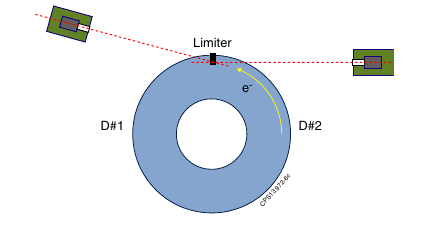
\includegraphics[width=0.72\linewidth]{tumanHxdDetectors} }
  \caption{ Расположение детекторов NaI(Tl) на токамаке Туман-3М.~\cite{Shevelev2013} }
  \label{fig:tumanHxdDetectors}
\end{figure}

Спектры жёсткого рентгеновского излучения, зарегистрированные детекторами 1 и 2 в процессе нарастания тока плазмы Туман-3М в разреженном (плотность $2-3 \times 10^{19}$~м${}^{-3}$) разряде, показаны на рисунках~\ref{fig:tumanHxdSpectrumsEdf}, (a) и (b) чёрными точками. Оба спектра наблюдают одно и то же место на лимиттере, различие в спектрах обусловлено различием в направлении наблюдения. Затем из спектра, измеренного детектором~1, была восстановлена функция распределения электронов по энергии. Она показана на рисунке~\ref{fig:tumanHxdSpectrumsEdf} (c). При восстановлении никак не использовалась информация с детектора~2. По полученной таким образом функции распределения были обратно рассчитаны спектры жёсткого рентгена для детекторов 1 и 2, которые показаны рисунках~\ref{fig:tumanHxdSpectrumsEdf}, (a) и (b) синими линиями. Видно, что рассчитанные таким образом спектры очень близки к экспериментальным. Для детектора~1 такое совпадение ожидаемо, поскольку для получения функции распределения использовался спектр с этого детектора в качестве исходных данных. Информация с детектора~2 не использовалась при получении функции распределения, однако и для него видно очень хорошее совпадение экспериментального и вычисленного спектров. Это может свидетельствовать о корректности всей процедуры --- как расчёта аппаратных функций и функций генерации излучения, так и собственно процедуры восстановления.~\cite{Shevelev2013}

\begin{figure}[ht!]
  \centerfloat{ 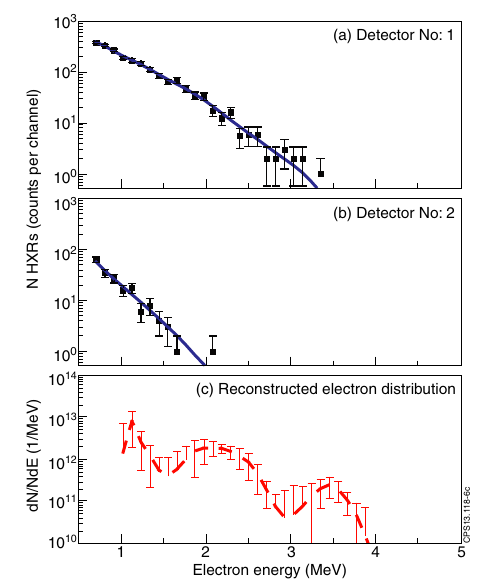
\includegraphics[width=0.52\linewidth]{tumanHxdSpectrumsEdf} }
  \caption{ a --- спектр, измеренный с помощью детектора~1; b --- спектр, измеренный с помощью детектора~2; c --- восстановленная функция распределения убегающих электронов по энергии. На рисунках (a) и (b) чёрными точками показан измеренный спектр, синий линией --- спектр излучения, соответствующий функции распределения, изображённой на рисунке (c).~\cite{Shevelev2013} }
  \label{fig:tumanHxdSpectrumsEdf}
\end{figure}

Стоит отметить, что было бы интересно восстановить функцию распределения убегающих электронов независимо с детекторов 1 и 2, и сравнивать уже сами функции распределения. Однако для более-менее корректного восстановления требуется достаточная статистика измеренных спектров. Для используемых на токамаке Туман-3М детекторов NaI(Tl) почти невозможно получить хорошую статистику на обоих детекторах: или на одном из детекторов она будет достаточно хорошей, а на другом --- недостаточной, или на втором она будет достаточной, но тогда загрузка первого детектора окажется чрезвычайно большой, и построить спектр окажется практически невозможно. 

% ----------------------------------------------------------

\subsection{ Влияние статистики и загрузки детектора на результаты восстановления функции распределения }

Очевидно что точность восстановления функции распределения будет зависеть от статистики измеренного спектра. На рисунке~\ref{fig:ft2TestReStatistics} представлены смоделированные спектры жесткого рентгеновского излучения. Исходная модельная функция распределения имела колокообразный профиль с максимальной энергией 8~МэВ, показанный на правых рисунках (d)--(f) красными линиями. Использовались функции отклика детектора LaBr3(Ce) $\varnothing$25.4$\times$76.2~мм, с помощью которого проводились измерения на токамаке ФТ-2; они показаны на рисунке~\ref{fig:ft2HxrDetectrorsAndReResponse}~(а). Были использованы функции генерации излучения убегающими электронами, соответствующие условиям токамака ФТ-2; они показаны на рисунке~\ref{fig:ft2HxrDetectrorsAndReResponse}~(б). После вычисления спектра на него был наложен пуассоновский шум. Полный интеграл числа событий в модельном спектре составлял $10^3$, b) $10^4$ и c) $10^5$~событий. Спектры показаны на рисунке~\ref{fig:ft2TestReStatistics} (a)--(c) чёрными точками.~\cite{Shevelev2016}

\begin{figure}[ht!]
    \begin{minipage}[b][][b]{0.45\linewidth}\centering
        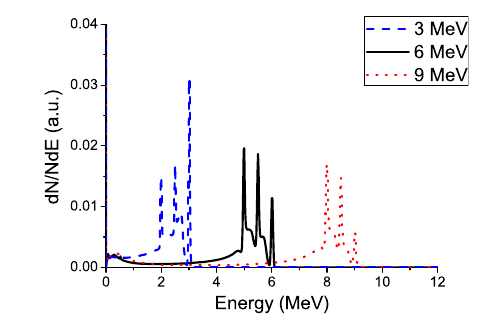
\includegraphics[width=0.92\linewidth]{ft2HxrDetectrorsResponse} \\ а) \\
    \end{minipage}
    \hfill
    \begin{minipage}[b][][b]{0.45\linewidth}\centering
        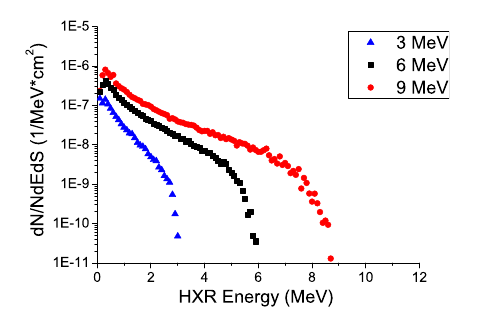
\includegraphics[width=0.92\linewidth]{ft2HxrReGenerationResponse} \\ б) \\
    \end{minipage}
    \vspace{5mm}
    \caption{ (а) --- отклик детектора LaBr3(Ce), использовавшегося в измерениях на токамаке ФТ-2, расчитанный кодом MCNP; (б) --- функции генерации тормозного жёсткого рентгеновского излучения убегающими электронами при взаимодействии с лимиттером, расчитанные кодом MCNP~\cite{Shevelev2016}. }
    \label{fig:ft2HxrDetectrorsAndReResponse}
\end{figure}

\begin{figure}[ht!]
  \centerfloat{ 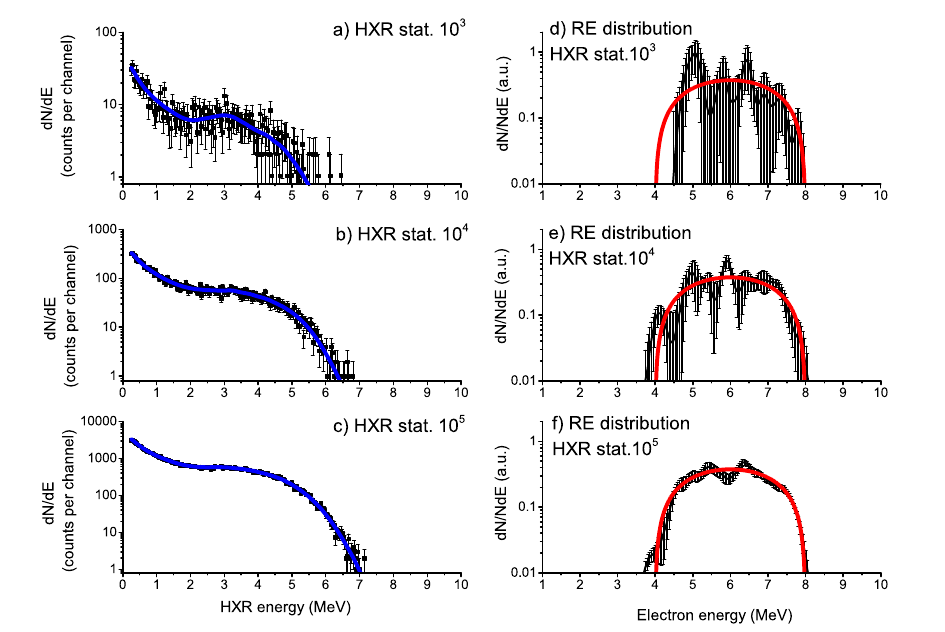
\includegraphics[width=0.95\linewidth]{ft2TestReStatistics} }
  \caption{ Левая колонка --- модельные спектры жёсткого рентгеновского излучения, сгенерированные с разной статистикой: a) $10^3$, b) $10^4$ и c) $10^5$~событий. Правая колонка --- результаты восстановления модельной функции распределения электронов для различной статистики спектров: d) $10^3$, e) $10^4$ и f) $10^5$~событий. Модельная функция распределения электронов показана красной линией, чёрная линия --- результат восстановления. На левых графиках чёрными точками показаны сгенреированные спектры, синими линиями показаны свертки полученных в результате восстановления электронных распределений с функцией отклика детектора и функцией генерации излучения.~\cite{Shevelev2016} }
  \label{fig:ft2TestReStatistics}
\end{figure}

Результат восстановления функции распределения по сгенерированным спектрам показан на рисунке~\ref{fig:ft2TestReStatistics} (d)--(f) чёрными линиями. Синие линии на левых графиках представляют собой свертки полученных распределений с функцией отклика детектора и функцией генерации излучения. На спектрах виден эффект улучшения результатов восстановления с улучшением статистики. Даже при низкой статистике в $10^3$~событий удалось корректно описать правый край функции распределения, а так же получить общую форму функции распределения. Отметим, что в экспериментах обычно статистика спектра лежит в исследуемом диапазоне $10^3$--$10^5$ событий в спектре~\cite{Shevelev2016}

Обращает на себя внимание то, что максимальная энергия зарегистрированных квантов жёсткого рентгеновского излучения оказывается всегда меньше чем максимальная энергия убегающих электронов. Разница между максимальной энергией квантов излучения и максимальной энергией электронов тем больше, чем меньше статистика спектра. Это обусловлено сильно спадающим характером функции генерации излучения убегающими электронами, который хорошо виден на рисунках~\ref{fig:mcnpRunawayResponseJetSh2013} и \ref{fig:ft2HxrDetectrorsAndReResponse}.~\cite{Shevelev2016}

%Так же отметим, что использовавшийся в старых работах метод определения максимальной энергии убегающих электронов по 

Для исследования влияния скорости счёта на процедуру восстановления функции распределения были сгенерированы модельные осциллограммы с различной загрузкой детектора. Генерация проводилась методом, описанным в разделе~\ref{sec:SignalGeneration}. Были сгенерированы осциллограммы, соответствующие разной скоростью счёта детектора ($10^5$, $10^6$, $3\times10^6$, $10^7$~с${}^{-1}$) с распределением событий по амплитуде, соответствующим исходному распределению убегающих электронов по энергии. Затем эти осциллограммы были обработаны методом фиттинга (раздел~\ref{sec:FittingProcessing}), были построены спектры, которые были обработаны в соответствии с процедурой из раздела~\ref{sec:runawayReconstructionMlem} для восстановления функции распределения убегающих электронов по энергии. Сравнение исходной сгенерированной функции распределения и восстановленной функции распределения показано на рисунке~\ref{fig:ft2TestReCountRate}.~\cite{Shevelev2016}


\begin{figure}[ht!]
  \centerfloat{ 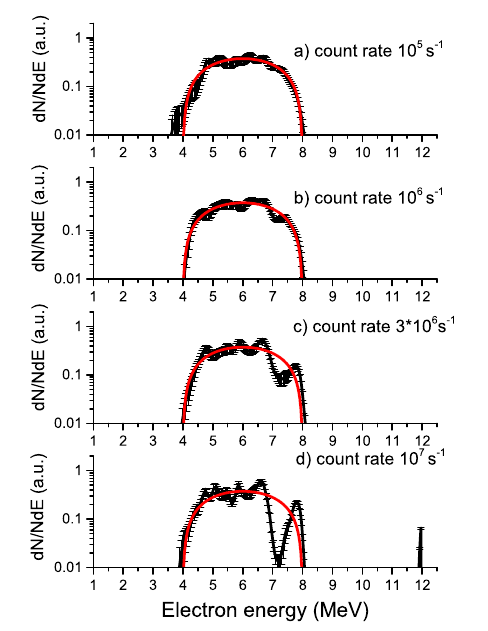
\includegraphics[width=0.95\linewidth]{ft2TestReCountRate} }
  \caption{ Восстановление функции распределения по модельным осциллограммам, соответствующим различной загрузке детектора. Красной линией показана сгенерированная осциллограмма, чёрной --- восстановленная из сгенерированного спектра.~\cite{Shevelev2016} }
  \label{fig:ft2TestReCountRate}
\end{figure}

При увеличении загрузки детектора улучшается статистика спектра и, соответственно, улучшается качество восстановления функции распределения. С другой стороны, при увеличении загрузки детектора растёт и количество наложенных импульсов на осциллограмме, что приводит к искажениям измеренного спектра (уменьшение доли низких квантов жёсткого рентгена и наоборот появлению ложных высокоэнергетичных событий). В свою очередь это приводит к аретфактам при восстановлении функции распределения. Тем не менее, отметим что максимальная энергия восстановленного распределения убегающих электронов смещается всего на 100--150~кэВ. Видно что при загрузке $10^7$~событий в секунду в области высоких энергий появлялся паразитный пик (однако число электронов в этом пике не превышает 0.5\% от общего распределения, и поэтому этот эффект следует считать пренебрежимо малым). Следует отметить, что при скорости счета детектора выше $10^7$~с${}^{-1}$ измеряемые спектры могут быть искажены из-за насыщения ФЭУ~\cite{Loher20121}, однако в моделировании этот эффект не учитывался.~\cite{Shevelev2016}

Таким образом, проведенный анализ смоделированных спектров жёсткого рентгеновского излучения с различной нагрузкой детектора и статистикой показал, что спектры, измеренные разработанным спектрометром LaBr 3(Ce) при скоростях счета до нескольких МГц, могут быть использованы для восстановления распределения энергии убегающих электронов во времени. В некоторых случаях восстановление полной функции распределения энергии убегающих электронов может привести к некоторым артефактам, которые следует тщательно анализировать. 

% ----------------------------------------------------------

\section{Выводы к главе 3}

Рассмотрено применение алгоритма ML-EM для восстановления спектра гамма излучения источников по измеренному с помощью сцинтилляционных детекторов спектру излучения. Для проведения процедуры восстановления требуется вычислить аппаратную функцию детектора и то, как ослабляется поток гамма квантов на пути от источника к детектору. Это вычисление может быть выполнено кодом MCNP. Был предложен ряд модификаций для адаптации базового алгоритма к условиям, которые имеются в задачах гамма-спектрометрии. Для вычисления погрешности восстановленного спектра предлагается использовать метод Монте-Карло.

Для проверки корректности процедуры восстановления были проведены эксперименты с калибровочными источниками ${}^{60}$Co и ${}^{137}$Cs излучения известной интенсивности. По восстановленным спектрам была рассчитана активность источников, которая совпала с точностью 1.5\% при обработке измеренного спектра с большой статистикой (время набора 300~с, расстояние до источника 25.5~см) и с точностью 2.5\% при обработке измеренного спектра с малой статистикой (время набора 2~с, расстояние до источника 25.5~см). Так же был проведён эксперимент с источником ${}^{152}$Eu, особенностью которого является наличие большого числа линий на спектре. В ходе восстановления удалось идентифицировать линии, в том числе не разрешённые на исходном измеренном спектре, и определить их интенсивность.  

Показано, что алгоритм ML-EM с модификациями применим для восстановления функции распределения убегающих электронов по энергии по измеренному спектру тормозного жёсткого рентгеновского излучения. Предложен метод определения максимальной энергии убегающих электронов по восстановленной функции распределения. 

Для проверки корректности процедуры восстановления функции распределения были проведены численные эксперименты. Было исследовано влияние статистики спектра и загрузки детектора на восстановленную функцию распределения. Показано, что при статистике спектра $10^3$ -- $10^5$~с${}^{-1}$ восстановленная функция соответствует исходной; показано, что при загрузке детектора $3 \times 10^6$~с${}^{-1}$ и выше восстановленная функция распределения оказывается искажённой из-за влияния наложений при обработке осциллограммы, однако в целом так же передаёт характер исходной функции распределения. Кроме того, для проверки процедуры восстановления были использованы результаты экспериментов на токамаке Туман-3М. В ходе этих экспериментов с помощью двух независимых детекторов измерялся спектр жёсткого рентгеновского излучения из одной и той же точки лимиттера, затем были проведены процедуры восстановления и сравнения, которые показали хорошее согласование результатов, полученных с различных независимых детекторов.

% ==========================================================

\FloatBarrier
